\documentclass[a4paper, 10pt]{memoir}

\let\leftbar\undefined
\let\endleftbar\undefined
\usepackage[nothm]{thmbox}
\let\proof\undefined\let\endproof\undefined

\usepackage[T1]{fontenc}
\usepackage[french,english]{babel}
\selectlanguage{english}
\usepackage[utf8]{inputenc}
\usepackage{mathbbol} %permet \mathbb{1} \Lbrack \Rbrack ...
\usepackage{amsmath,amssymb,amsthm,amsfonts} %packages AMS
\usepackage{wasysym}
\usepackage{calrsfs} %\mathcal{} plus rondes
\usepackage{enumerate} %permet de changer le type de numérotation
                       %dans enumerate
\usepackage{graphicx} %permet d'afficher des images
\usepackage{titlesec,titletoc} %modifie les titres et la table des matières
\usepackage{lettrine} %permet les lettrines
\usepackage{todonotes}
\PassOptionsToPackage{hyphens}{url}
\usepackage[style=alphabetic,backref=true]{biblatex}
\renewbibmacro{in:}{}
\usepackage[colorlinks=true,linkcolor=black,urlcolor=blue,citecolor=gray]{hyperref}
\usepackage{csquotes}
\bibliography{biblio}
\usepackage{mathpazo}
\linespread{1.05}
\usepackage{lipsum}
\setlipsumdefault{1-4}


\usepackage{adjustbox}
\usepackage{graphicx}




\tolerance 1414
\hbadness 1414
\emergencystretch 1.5em
\hfuzz 0.3pt
\widowpenalty=10000
\vfuzz \hfuzz
\raggedbottom

\newtheoremstyle{theoreme}
 {2em} %espace avant le théorème
 {2em} %espace après le théorème
 {\slshape} %fonte du texte
 {} %indentation
 {\bfseries} %fonte du titre
 {} %ponctuation après le titre
 {\newline} %espace après le titre
 {\thmname{#1}\thmnumber{ #2}\thmnote{~:~#3}} %forme du titre


\theoremstyle{theoreme} 
\newtheorem{thm}{Theorem}[chapter]
\newtheorem{cor}[thm]{Corollary}
\newtheorem{prop}[thm]{Proposition}
\newtheorem{defi}[thm]{Definition}
\newtheorem{lem}[thm]{Lemma}
\newtheorem{cond}[thm]{Condition}
\newtheorem{ax}[thm]{Axiom}

\newtheorem{thmfr}{Théoreme}[chapter]
\newtheorem{corfr}[thm]{Corollaire}
\newtheorem{defifr}[thm]{Définition}
\newtheorem{lemfr}[thm]{Lemme}
\newtheorem{axfr}[thm]{Axiome}

\newenvironment{prooflem}%
    {\renewcommand{\qedsymbol}{$\Diamond$}%
     \begin{proof}}%
    {\end{proof}%
     \renewcommand{\qedsymbol}{$\square$}}

% \newenvironment{rmq}% 
% 	{\noindent \textsc{Nota}~\textendash~}%
% 	{\medskip}

% \newenvironment{exm}%
% 	{\noindent \textsc{Example}~\textendash~}%
% 	{\medskip}

\newenvironment{rmqs}%
	{\noindent \textsc{Notae}~:~ \medskip%
	 \begin{list}%
		{\textendash}%
		{\setlength{\itemsep}{2ex}}}%
	{\end{list} \medskip}

\newenvironment{exms}%
	{\noindent \textsc{Examples}~:~ \medskip%
	 \begin{list}%
		{\textendash}%
		{\setlength{\itemsep}{2ex}}}%
	{\end{list} \medskip}

\newenvironment{nota}% 
	{\noindent \textsc{Notation}~\textendash~}%
	{\medskip}

%% Maths %%

        % HoTT %
\usepackage[all]{xy}
\def\dar[#1]#2{\ar@<-#2>[#1]\ar@<#2>[#1]} %double arrows in xy
\def\tar[#1]#2{\ar@<#2>[#1]\ar@<0pt>[#1]\ar@<-#2>[#1]} %triple arrows in xy
\DeclareMathOperator{\Type}{Type}
\DeclareMathOperator{\HProp}{HProp}
\DeclareMathOperator{\HSet}{HSet}
\DeclareMathOperator{\IsHProp}{IsHProp}
\DeclareMathOperator{\IsHSet}{IsHSet}
\DeclareMathOperator{\nat}{nat}
\DeclareMathOperator{\Unit}{Unit}
\DeclareMathOperator{\im}{Im}
\DeclareMathOperator{\id}{id}
\DeclareMathOperator{\Contr}{Contr}
\DeclareMathOperator{\IsContr}{IsContr}
\DeclareMathOperator{\IsEquiv}{IsEquiv}
\DeclareMathOperator{\precompose}{\mathrm{precompose}}
\DeclareMathOperator{\postcompose}{\mathrm{postcompose}}
\DeclareMathOperator{\idmap}{\mathrm{idmap}}
\DeclareMathOperator{\cocone}{cocone}
\DeclareMathOperator{\inl}{inl}
\DeclareMathOperator{\inr}{inr}
\DeclareMathOperator{\transport}{transport}
\DeclareMathOperator{\tr}{tr}
\DeclareMathOperator{\Sym}{Sym}
\DeclareMathOperator{\Trans}{Trans}
\DeclareMathOperator{\Refl}{Refl}


\newcommand \defeq {\overset{de\hspace{-0.2ex}f}{=}}

\def\mymathhyphen{{\hbox{-}}}

\newcommand{\IsType}[1]
{\mathop{\mathrm{Is\mymathhyphen}#1\mathrm{\mymathhyphen type}} }

\newcommand{\modal}{\ensuremath{\ocircle}}
\newcommand \True {\top}
\newcommand \idpath {\mathrm{idpath}}
\newcommand \False {\bot}
\newcommand \closure[1] {\overline{#1}}
\newcommand \Char[1] {\chi_{#1}}%{\mathrm{char}(#1)}
\newcommand \E {\mathcal{E}}
\newcommand \Hom[1] {\mathrm{Hom}_{#1}}
\newcommand \Obj {\mathrm{Obj}}
\newcommand \Sh[1] {\mathrm{Sh}_{#1}}
\newcommand \squash[1] {\| #1 \| }
\newcommand \separated {\mathop{\square_{n+1}} }
\newcommand \fib[2] {\mathrm{fib}_{#1}(#2)}
\newcommand \colim {\mathrm{colim}}
\newcommand \zero {\mathbf{0}}
\newcommand \one {\mathbf{1}}
\newcommand \unittt{\star}
\newcommand \two {\mathbf{2}}
\newcommand{\sumD}[3]{\sum_{#1:#2}\, #3}
\newcommand{\prodD}[3]{\prod_{#1:#2}\, #3}
\newcommand{\homot}{\sim}
\newcommand{\retr}{\mathrm{retr}}
\newcommand{\sect}{\mathrm{sect}}
\newcommand{\adj}{\mathrm{adj}}
\newcommand{\ap}[1]{\mathrm{ap}_{#1}}
\newcommand{\inv}[1]{#1^{-1}}
\newcommand{\concat}[2]{#1\cdot #2}
\newcommand{\happly}{\mathrm{happly}}
\newcommand{\Sone}{\mathbb{S}^1}
\newcommand{\baseS}{\mathrm{base}}
\newcommand{\loopS}{\mathrm{loop}}
\newcommand{\coeq}[2]{\mathrm{Coeq}^{#1,#2}}

\DeclareMathOperator{\issep}{IsSeparated}
\DeclareMathOperator{\issheaf}{IsSheaf}
\DeclareMathOperator{\KP}{KP}
\DeclareMathOperator{\kp}{kp}

	% Différentielles %
\newcommand{\diff}[1]{\mathrm{d}#1} %élément différentiel
\newcommand{\dpart}[2]{\frac{\partial #1}{\partial #2}} %dérivée partielle d'ordre 1

	% Ensembles %
\newcommand{\N}{\mathbb{N}} %entiers naturels
\newcommand{\R}{\mathbb{R}} %réels
\newcommand{\Q}{\mathbb{Q}} %rationnels
\newcommand{\Z}{\mathbb{Z}} %entiers relatifs
\newcommand{\C}{\mathbb{C}} %complexe
\newcommand{\K}{\mathbb{K}} %corps
\newcommand{\perm}{\mathfrak{S}} %permutations

        % Flèches %
\newcommand{\To}{\Rightarrow}
\newcommand{\ot}{\leftarrow}
\newcommand{\oT}{\Leftarrow}
\newcommand{\tot}{\leftrightarrow}
\newcommand{\ToT}{\Leftrightarrow}
\newcommand{\cto}{\hookrightarrow}
%\newcommand{\cot}{\hookleftarrow}



	% Fonctions %
\newcommand{\fonction}[5]{ %{nom de la fonction}{ensemble de départ}{ensemble d'arrivée}{nom de la variable}{image de la variable}
	#1 \, \colon \left.
	 \begin{array}{ccl}
		#2 & \longrightarrow & #3 \\
		#4 & \longmapsto & #5
	\end{array}
	\right.
}

\def\restriction#1#2{\mathchoice %restriction d'une fonction à un ensemble
              {\setbox1\hbox{${\displaystyle #1}_{\scriptstyle #2}$}
              \restrictionaux{#1}{#2}}
              {\setbox1\hbox{${\textstyle #1}_{\scriptstyle #2}$}
              \restrictionaux{#1}{#2}}
              {\setbox1\hbox{${\scriptstyle #1}_{\scriptscriptstyle #2}$}
              \restrictionaux{#1}{#2}}
              {\setbox1\hbox{${\scriptscriptstyle #1}_{\scriptscriptstyle #2}$}
              \restrictionaux{#1}{#2}}}
\def\restrictionaux#1#2{{#1\,\smash{\vrule height .8\ht1 depth .85\dp1}}_{\,#2}} 

	% Opérateurs %
\DeclareMathOperator{\rk}{Rk} %rang
\DeclareMathOperator{\vect}{Vect} %espace vectoriel engendré
\DeclareMathOperator{\mat}{mat} %matrice
\DeclareMathOperator{\Ker}{Ker} %noyau
\DeclareMathOperator{\diag}{diag} %matrice diagonale
\DeclareMathOperator{\jac}{Jac} %jacobien


\newcommand*{\EnsQ}[2]%
{\ensuremath{%
   \raisebox{.32ex}{\ensuremath{#1}}/\!\raisebox{-.60ex}{\ensuremath{#2}}}}


 % Lettrines %
\renewcommand{\LettrineFontHook}{\fontfamily{yfrak} \selectfont \color[gray]{0.7}}

\newenvironment{fracarray}[1]%
{\renewcommand{\arraystretch}{1.4}%
 \begin{array}{#1}%
}%
{\end{array}%
 \renewcommand{\arraystretch}{1}%
}

\newcommand{\ie}{\emph{i.e.}}
\newcommand{\eg}{\emph{e.g.}}
\newcommand{\etc}{\emph{etc.}}


\newenvironment{rmq}
{\begin{thmbox}[M]{\textsc{Nota}}\noindent}
{\end{thmbox}\medskip}

\newenvironment{exm}
{\begin{thmbox}[M]{\textsc{Example}}\noindent}
{\end{thmbox}\medskip}

\newenvironment{exmfr}
{\begin{thmbox}[M]{\textsc{Exemple}}\noindent}
{\end{thmbox}\medskip}


\usepackage[refpage, intoc]{nomencl}
\makenomenclature

\usepackage{bussproofs}
\setcounter{tocdepth}{2}
\setsecnumdepth{subsection}

\usepackage{nicefrac}

\author{Kevin \textsc{Quirin}}
\title{Lawvere-Tierney Sheafification in Homotopy Type Theory}
\date{2016}

%Chapter Page
\usepackage[T1]{fontenc}
\usepackage{kpfonts}
\setSingleSpace{1.1}
\SingleSpacing
\usepackage{xcolor,calc}
\definecolor{chaptercolor}{gray}{0.8}
% helper macros
\newcommand\numlifter[1]{\raisebox{-2cm}[0pt][0pt]{\smash{#1}}}
\newcommand\numindent{\kern37pt}
\newlength\chaptertitleboxheight
\makechapterstyle{hansen}{
\renewcommand\printchaptername{\raggedleft}
\renewcommand\printchapternum{%
\begingroup%
\leavevmode%
\chapnumfont%
\strut%
\numlifter{\thechapter}%
\numindent%
\endgroup%
}
\renewcommand*{\printchapternonum}{%
\vphantom{\begingroup%
\leavevmode%
\chapnumfont%
\numlifter{\vphantom{9}}%
\numindent%
\endgroup}
\afterchapternum}
\setlength\midchapskip{0pt}
\setlength\beforechapskip{0.5\baselineskip}
\setlength{\afterchapskip}{3\baselineskip}
\renewcommand\chapnumfont{%
\fontsize{4cm}{0cm}%
\bfseries%
\sffamily%
\color{chaptercolor}%
}
\renewcommand\chaptitlefont{%
\normalfont%
\huge%
\bfseries%
\raggedleft%
}%
\settototalheight\chaptertitleboxheight{%
\parbox{\textwidth}{\chaptitlefont \strut bg\\bg\strut}}
\renewcommand\printchaptertitle[1]{%
\parbox[t][\chaptertitleboxheight][t]{\textwidth}{%
%\microtypesetup{protrusion=false}% add this if you use microtype
\chaptitlefont\strut ##1\strut}%
}
}
\chapterstyle{hansen}

%% Titlepage

% \newlength\dropp
% \makeatletter
% \newcommand*{\titleDS}{\begingroup% DS Thesis
% \dropp=0.1\textheight
% %\vspace*{\drop}
% \centering
% {\Large\bfseries Lawvere-Tierney Sheafification in Homotopy Type Theory}\par
% \vspace{0.6\baselineskip}
% {By}\\[0.6\baselineskip]
% {Kevin~Quirin\\[0.6\baselineskip]
% %A Thesis Submitted to the Graduate\\[0.5\baselineskip]
% %Faculty of The University\\[0.5\baselineskip]
% %in Partial Fulfillment of the\\[0.5\baselineskip]
% %Requirements for the Degree of\\[0.5\baselineskip]
% %DEGREE\\[0.5\baselineskip]
% Major Subject: Computer Science}\par
% \flushleft
% {Approved by the \\
% Examining Committee:}\par
% \vspace{1.5\baselineskip}
% \rule{15em}{0.4pt}\\
% Pierre Cointe, Thesis Advisor \\[1\baselineskip]
% \rule{15em}{0.4pt}\\
% Nicolas Tabareau, Thesis Advisor \\[1\baselineskip]
% \rule{15em}{0.4pt}\\
% Carl F. Gau\ss, Göttingen\\[1\baselineskip]
% \rule{15em}{0.4pt}\\
% Euclid, Athens \\[1\baselineskip]
% \centering
% \vspace{1\baselineskip}
% Mines de Nantes \\
% [\baselineskip]
% 2016\par 
% \vfill
% \endgroup}
% \makeatother


\def\pullbackcorner{%
    \ar@{-}[]+R+<6pt,-1pt>;[]+RD+<6pt,-6pt>%
    \ar@{-}[]+D+<1pt,-6pt>;[]+RD+<6pt,-6pt>%
  }

\newcommand{\code}[1]{\texttt{#1}}

\usepackage[a4paper]{geometry}

\definecolor{@doctoratcolor}{RGB}{91, 91, 91}
      \definecolor{@verticalgreen}{RGB}{238, 238, 238}
      \definecolor{@horizontalgray}{gray}{0.97265}
      \definecolor{@textgray}{gray}{0.5}
      \definecolor{@bandeaucolor}{RGB}{190, 190, 190}
      \definecolor{@titlecolor}{RGB}{116, 116, 116}
\newcommand{\Hugecover}{\fontsize{25}{30}\selectfont}
\newcommand{\hugecover}{\fontsize{25}{30}\selectfont}
\newcommand{\LARGEcover}{\fontsize{20}{25}\selectfont}
\newcommand{\Largecover}{\fontsize{17}{22}\selectfont}
\newcommand{\normalsizecover}{\fontsize{12}{14.5}\selectfont}
\newcommand{\smallcover}{\fontsize{11}{13.6}\selectfont}
\newcommand{\footnotesizecover}{\fontsize{10}{12}\selectfont}
\newcommand{\scriptsizecover}{\fontsize{8}{9.5}\selectfont}
\newcommand{\tinysizecover}{\fontsize{6}{7}\selectfont}

\DisemulatePackage{setspace}
\usepackage{setspace}

\makeatletter
\newcommand{\@drawbackground}
   { % Horizontal grey-green box
   \noindent\raisebox{0pt}[0pt][0pt]
                     {\colorbox{@verticalgreen}
                               {\makebox[0.5\textwidth]
                                        {\raisebox{-\textheight}
                                                  {~}}}}

   \vspace{4\baselineskip}

   {
   \noindent\hspace{0.45\textwidth}
            \raisebox{0pt}[0pt][0pt]
                     {\color{@horizontalgray}
                      \rule{0.55\textwidth}
                           {2.5\baselineskip}}
            \hspace{-0.45\textwidth}
   }

   \renewcommand{\sfdefault}{phv}
   \renewcommand{\rmdefault}{ptm}
   \renewcommand{\ttdefault}{pcr}
   \sffamily
   \fontsize{12pt}{14pt}
   \selectfont

   \noindent\makebox[0.55\textwidth][r]
                    {\Hugecover\textbf{\textcolor{@doctoratcolor}
                                                 {Th\`ese de Doctorat}}}

   {
   \noindent\color{@bandeaucolor}
            \rule{0.55\textwidth}
                 {2.5\baselineskip}
            \color{@horizontalgray}
            \rule{0.45\textwidth}
                 {2.5\baselineskip}
   }

   \vspace{3\baselineskip}

   {
   \noindent\hspace{0.45\textwidth}
            \raisebox{0pt}[0pt][0pt]
                     {\color{@horizontalgray}
                      \rule{0.55\textwidth}
                           {2.5\baselineskip}}
            \hspace{-0.45\textwidth}
   }

   \vspace{-15\baselineskip}
   
\includegraphics[width=4.5cm]{logos/LUNAM-CUE}
   \hfill
   \hfill
   \hfill
   \ifx\@cosupervisingforeigninstitution\@empty
   \else
   %    \raisebox{\@cosupervisingforeigninstitutionlogovoffset}[0pt][0pt]{\includegraphics[width=\@cosupervisingforeigninstitutionlogowidth]{logos/\@cosupervisingforeigninstitutionlogo}}~
   %    \hfill
   % \fi
   % \ifx\@coinstitution\@empty
   % \else
   % \global\let\@coinstitutionlogovoffset{10pt}
   % \raisebox{\@coinstitutionlogovoffset}[0pt][0pt]{
\includegraphics[width=\@coinstitutionlogowidth]{logos/MinesNantes}}~
   % \hfill
   % \fi
   \raisebox{0pt}[0pt][0pt]{
\includegraphics[width=2.4cm]{logos/MinesNantes}}~
   \vspace{11\baselineskip}
 }
\makeatother

\makeatletter
\newcommand{\@committee}{%
  \noindent
  \begin{tabular}{ll}
    \footnotesizecover%
    {Rapporteurs}  &  {\textbf{M. John Doe}, Professor, University of Mordor} \\
                   &  {\textbf{M. John Doe}, Professor, University of Mordor} \\
    {Examinateurs} &  {\textbf{M. John Doe}, Professor, University of Mordor} \\
                   &  {\textbf{M. John Doe}, Professor, University of Mordor} \\
    {Directeur de thèse} & {\textbf{M. Pierre Cointe}, Professeur,
                           École des Mines de Nantes} \\
    {Co-directeur de thèse} & {\textbf{M. Nicolas Tabareau}, Chargé de
                              recherche, Inria Rennes-Bretagne-Atlantique}
   \end{tabular}}
\makeatother



\makeatletter

%%%%%%%%%%%%%%%%%%%%%%%%%%%
% R'esum'e en franc,ais
%

\newsavebox{\@resumeBox}
\newbox{\@resumeBoxGlobal}

\newenvironment{resume}
   {
   \newgeometry{margin=1.5cm}
   \begin{lrbox}{\@resumeBox}%
      \renewcommand{\sfdefault}{phv}
      \renewcommand{\rmdefault}{ptm}
      \renewcommand{\ttdefault}{pcr}
      \smallcover\sffamily
      \begin{minipage}{0.47\textwidth}
         \begin{flushleft}
            \selectlanguage{french}
            \textbf{R\'esum\'e}\par
   }
   {
         \end{flushleft}
      \end{minipage}
   \end{lrbox}
   \restoregeometry
   \global\setbox\@resumeBoxGlobal=\vbox{\copy\@resumeBox}
   }

%%%%%%%%%%%%%%%%%%%%%%%%
% R'esum'e en anglais
%

\newsavebox{\@abstractBox}
\newbox{\@abstractBoxGlobal}

\newenvironment{abstract_}
   {
   \newgeometry{margin=1.5cm}
   \begin{lrbox}{\@abstractBox}%
      \renewcommand{\sfdefault}{phv}
      \renewcommand{\rmdefault}{ptm}
      \renewcommand{\ttdefault}{pcr}
      \smallcover\sffamily
      \begin{minipage}{0.47\textwidth}
         \begin{flushleft}
            \selectlanguage{english}
            \textbf{Abstract}\par
   }
   {
         \end{flushleft}
      \end{minipage}
   \end{lrbox}
   \restoregeometry
   \global\setbox\@abstractBoxGlobal=\vbox{\copy\@abstractBox}
   }

%%%%%%%%%%%%%%%%%%%%%%%%%%%%
% Mots cl'es en franc,ais
%

\newsavebox{\@keywordsBox}
\newbox{\@keywordsBoxGlobal}

\newenvironment{keywords}
   {
   \newgeometry{margin=1.5cm}
   \begin{lrbox}{\@keywordsBox}%
      \renewcommand{\sfdefault}{phv}
      \renewcommand{\rmdefault}{ptm}
      \renewcommand{\ttdefault}{pcr}
      \smallcover\sffamily
      \begin{minipage}{0.47\textwidth}
         \begin{flushleft}
            \selectlanguage{english}
            \textbf{Key Words}\par
   }
   {
         \end{flushleft}
      \end{minipage}
   \end{lrbox}
   \restoregeometry
   \global\setbox\@keywordsBoxGlobal=\vbox{\copy\@keywordsBox}
   }

%%%%%%%%%%%%%%%%%%%%%%%%%
% Mots cl'es en anglais
%

\newsavebox{\@motsclesBox}
\newbox{\@motsclesBoxGlobal}

\newenvironment{motscles}
   {
   \newgeometry{margin=1.5cm}
   \begin{lrbox}{\@motsclesBox}%
      \renewcommand{\sfdefault}{phv}
      \renewcommand{\rmdefault}{ptm}
      \renewcommand{\ttdefault}{pcr}
      \smallcover\sffamily
      \begin{minipage}{0.47\textwidth}
         \begin{flushleft}
            \selectlanguage{french}
            \textbf{Mots cl\'es}\par
   }
   {
         \end{flushleft}
      \end{minipage}
   \end{lrbox}
   \restoregeometry
   \global\setbox\@motsclesBoxGlobal=\vbox{\copy\@motsclesBox}
   }

\global\newcount\@startingPage

\newcommand{\makecover}{%
   \singlespacing
   \newgeometry{margin=1.5cm}
   \cleardoublepage % go to odd page
   \phantom{placeholder} % doesn't appear on page
   \newpage % on even page
   \thispagestyle{empty} % no numbering
   \@startingPage\thepage\relax
      {
      \@drawbackground
      \vspace{-5.5\baselineskip}
      \renewcommand{\sfdefault}{phv}
      \renewcommand{\rmdefault}{ptm}
      \renewcommand{\ttdefault}{pcr}
      \sffamily
      \fontsize{12pt}{14pt}
      \selectfont
      \begin{quote}
         \begin{flushleft}
            \textbf{\Largecover\textcolor{@textgray}{Kevin\textsc{Quirin}}}
         \end{flushleft}

         \begin{flushleft}
            \textbf{\textcolor{@textgray}{Faisceautisation de
                Lawvere-Tierney en théorie des types homotopiques}}
         \end{flushleft}
         \begin{flushleft}
            \textbf{\textcolor{@textgray}{Lawvere-Tierney
                sheafification in Homotopy Type Theory}}
         \end{flushleft}
      \end{quote}

      \vfill

      \noindent
      \hfill\parbox[t][][b]
            {0.47\textwidth}
            {\makebox[0.47\textwidth]{\usebox{\@resumeBoxGlobal}}}
      \hfill
      \hfill\parbox[t][][b]
            {0.47\textwidth}
            {\makebox[0.47\textwidth]{\usebox{\@abstractBoxGlobal}}}
      \hfill

      \vfill

      \noindent
      \hfill\parbox[t][][b]
            {0.47\textwidth}
            {\makebox[0.47\textwidth]{\usebox{\@motsclesBoxGlobal}}}
      \hfill
      \hfill\parbox[t][][b]
            {0.47\textwidth}
            {\makebox[0.47\textwidth]{\usebox{\@keywordsBoxGlobal}}}
      \hfill

      \vfill

      \hspace{0.45\textwidth}\raisebox{-2.2\baselineskip}
                                      [0pt][0pt]
                                      {\colorbox{@bandeaucolor}
                                                {\parbox[s]
                                                        [2\baselineskip]
                                                        [c]
                                                        {0.55\textwidth}
                                                        {~\hfill
                                                         \textcolor{white}
                                                                   {L'UNIVERSIT\'E NANTES ANGERS LE MANS}
                                                         \hfill~}}}%
      }%
   \restoregeometry%
} % \makecover
\makeatother

\AtEndDocument{\makecover}


\begin{document}

\begin{resume}
  Le but principal de cette thèse est de définir une extension de la
  traduction de double-négation de Gödel à tous les types tronqués,
  dans le contexte de la théorie des types homotopique.
  Ce but utilisera des théories déjà existantes, comme la théorie des
  faisceaux de Lawvere-Tierney, que nous adapterons à la théorie des
  types homotopiques. En particulier, on définira le fonction de
  faisceautisation de Lawvere-Tierney, qui est le principal théorème
  présenté dans cette thèse.

  Pour le définir, nous aurons besoin de concepts soit déjà définis
  en théorie des types, soit non existants pour l'instant. En
  particulier, on définira une théorie des colimits sur des graphes,
  ainsi que leur version tronquée, et une notion de modalités
  tronquées basée sur la définition existante de modalité.

  Presque tous les résultats présentés dans cette thèse sont
  formalisée avec l'assistant de preuve Coq, muni de la
  librairie~\cite{hottlib}.
\end{resume}

\begin{abstract_}
  The main goal of this thesis is to define an extension of Gödel
  not-not translation to all truncated types, in the setting of
  homotopy type theory. 
  This goal will use some existing theories, like Lawvere-Tierney
  sheaves theory in toposes, we will adapt in the setting of homotopy
  type theory. In particular, we will define a Lawvere-Tierney
  sheafification functor, which is the main theorem presented in this
  thesis.

  To define it, we will need some concepts, either already defined in
  type theory, either not existing yet. In particular, we will define
  a theory of colimits over graphs as well as their truncated version,
  and the notion of truncated modalities, based on the existing
  definition of modalities.

  Almost all the result presented in this thesis are formalized with
  the proof assistant Coq together with the library~\cite{hottlib}.
\end{abstract_}

\begin{motscles}
  Théorie des types, homotopie, faisceautisation, Coq
\end{motscles}

\begin{keywords}
  Type theory, homotopy, sheafification, Coq
\end{keywords}


\newgeometry{margin=1.5cm}
\begin{titlingpage}
  {
    \singlespacing
    \makeatletter
    \@drawbackground
    \renewcommand{\sfdefault}{phv}
    \renewcommand{\rmdefault}{ptm}
    \renewcommand{\ttdefault}{pcr}
    \fontsize{12pt}{14pt}
    \sffamily
    \selectfont
    
    \vspace{-3.75\baselineskip}
    \hspace{0.5\textwidth}
    \raisebox{0pt}
    [0pt]
    [2\baselineskip]
    {\parbox[t][][c]
      {0.5\textwidth}
      {\raggedright\textcolor{@doctoratcolor}{\begin{spacing}{0.75}\Hugecover{Kevin \textsc{Quirin}}\end{spacing}}}}
    
    \smallcover
    \vspace{\baselineskip}
    
    \noindent\textsl{M\'emoire pr\'esent\'e en vue de l'obtention du}\par
    \noindent\textsl{\textbf{grade de Docteur
        de \parbox[t]{0.79\textwidth}{l'École nationale supérieure
          des Mines de Nantes}}}\par
    \noindent\textsl{\textbf{\phantom{grade de }Label européen}}\par
    \noindent\textsl{sous le label de l'Universit\'e de Nantes Angers Le Mans}\par
    
    \vspace{\baselineskip}
    
    \footnotesizecover
    \noindent\textbf{\'Ecole doctorale : Sciences et technologies de
      l'information, et mathématiques}\par
    
    \vspace{\baselineskip}
    
    \footnotesizecover
    \noindent\textbf{Discipline : Informatique et applications,
      section CNU 27}\par
    \noindent\textbf{Unit\'e de recherche
      : \parbox[t]{0.8\textwidth}{Laboratoire d'informatique de
        Nantes-Atlantique (LINA)}}\par
    
    \vspace{\baselineskip}
    
    \footnotesizecover
    \noindent\textbf{Soutenue le FIXME}\par
    \noindent\textbf{Th\`ese n\textdegree\ : FIXME}\par
    
    \vfill
    
    \hfill
    \parbox{0.75\textwidth}
    {\begin{flushright}
        \Largecover\textcolor{@titlecolor}{\textbf{Lawvere-Tierney
            sheafification in \\ Homotopy Type Theory}}\\
      \end{flushright}}
    
    \vfill
    \vfill
    \vfill
    
    \newsavebox{\@committeebox}
    \sbox{\@committeebox}{\@committee}
    \newlength{\committeeboxwidth}
    \settowidth{\committeeboxwidth}{\usebox{\@committeebox}}
    \begin{center}
      \textcolor{@titlecolor}{\textbf{\smallcover JURY}}\par
      \vspace{1em}
      {\centering\usebox{\@committeebox}}%
    \end{center}
  }
\end{titlingpage}%
\makeatother
\restoregeometry

\frontmatter%

\begin{abstract}
  \todo[inline]{Write the abstract}
\end{abstract}
\chapter{Acknowlegdments}

First of all, I would like to thank Nicolas Tabareau for the time he
spent helping me. All this thesis is also his work, and I would never
have finished it withour his help.
Without him, I would never have discovered homotopy type theory and
computer-checked proofs~; even worse, I would have become a set
theorist. Thank you again for avoiding this. 
I am also grateful to Matthieu and Tom for accepting to review my
wiork during three years~; these discussions were always helpful.
\bigskip

Special thanks also go to my thesis committee, Pierre Cointe, Mart\'in
Escard\'o, André Hirschowitz, Matthieu Sozeau and Bas Spitters. All
these names were for me role models during my PhD, and their presence
at the defense was an honor for me.
A huge amount of work has been done by the examiners of my thesis
Mart\'in Escard\'o and André Hirschowitz, and the  who spent a lot of time
reading carefully my words, and I can never thank them enough.

\bigskip

For all the type theoretic discussions at École des Mines de Nantes, I
want to thank Guilhem Jaber, Simon Boulier, Rafael Bocquet, Gabriel
Lewertowski, Pierre-Marie Pédrot, Benedikt Ahrens and
Egbert Rijke. For all the non-type theoretic discussions at École des
Mines de Nantes, I want to thank Florent, Ronan, Walid, Jonathan,
Anthony, Gustavo, Alexandre, Rémi, Hervé, and all the people living in
the computer science department.

\bigskip

It would never have been possible to write hundreds of lines of coherence
proofs without music, which played a major role in my work. For these
times, I thank Miles Davis, Metallica, Anonio Vivaldi, Led Zeppelin,
Yom, Sigur R\'os, Dead Weather, Arcade Fire and at least one thousand
more people. 

\bigskip

This work would not have been possible without the support of family
of friends, and I can never thank them enough for their support. I
won't give any names here, except Charlotte and Clémentine, who
inspire me every day.


% \todo[inline]{Write the acknowledgments}
%%% Local Variables:
%%% mode: latex
%%% TeX-master: "main"
%%% End:

\newpage
\tableofcontents

\mainmatter%
\begin{otherlanguage}{french}
  
\chapter{Résumé en français}

\section{Introduction}

La théorie des types homotopique est une branche nouvelle des
mathématiques et de l'informatique, exhibant un lien fort, mais
surprenant entre la théorie des $\omega$-catégories et la théorie de
types. Ce domaine se situe donc à la frontière entre les mathématiques
pures et l'informatique. Un des but de la recherche sur ce sujet est
d'utiliser la théorie des types homotopique comme une nouvelle
fondation des mathématiques, remplaçant par exemple la théorie des
ensembles de Zermelo-Fr\ae nkel. Ses liens forts avec la théorie des
types donneraient aux mathématiciens la possibilité de formaliser
leurs travaux avec un assistant de preuve comme
Coq~\cite{coq:refman:8.4}, Agda~\cite{norell2007towards} ou
Lean~\cite{lean}. En effet, les erreurs dans les articles de recherche
en mathématiques semblent inévitables~\cite{vv-univ-f}, et une preuve
vérifiée par ordinateur peut inspirer plus confiance qu'une preuve
vérifiée par un humain. Les exemples les plus célèbres de preuves
vérifiées par ordinateur sont le {\em théorème des quatre couleurs}
(pour colorier une carte telle qu'aucuns pays voisins aient la même 
couleur, il suffit de quatre couleurs) par Gonthier et
Werner~\cite{gonthier-four-color} avec Coq, le {\em théorème de
Feit-Thomson} (tout groupe fini d'ordre impair est résoluble) par
Gonthier et al.~\cite{gonthier-feit} avec Coq, la preuve originelle du 
{\em théorème de Jordan} (toute courbe simple continue fermée divise le plan
en une partie bornée ``intérieure'' et une partie non bornée
``extérieure'') par Hales~\cite{hales-jordan} avec Mizar, ou la {\em
  conjecture de Kepler} (les façons les plus compactes d'empiler des
sphères sont les empilements clos cubiques et hexagonaux) par Hales et
al.~\cite{hales-kepler} avec Isabelle et HOL Light.

Un des avantages de la théorie des types par rapport à la théorie des
ensembles est la propriété de calculabilité de la théorie des types :
tout terme est identifié avec sa forme normale. Ainsi, un assistant de
preuve permet à l'utilisateur de simplifier automatiquement toutes les
expressions, alors qu'une preuve sur papier requiert de faire toutes
ces calculs à la main. La théorie des ensembles ne partage pas cette
propriété de calculabilité, et n'est donc pas aussi pratique à
utiliser comme base théorique pour un assistant de preuve. Cependant,
cette propriété de calculabilité nous empêche d'utiliser des
propriétés classiques, telles que le tiers exclu ; en général, il est
impossible de prouver qu'une proposition est soit vraie, soit fausse.

L'ingrédient principal de la théorie des types homotopique, faisant le
lien entre les mathématiques et l'informatique, est l'isomorphisme de
Curry-Howard: on peut indifféremment parler de preuve ou de programme,
les deux décrivent les mêmes objets {\em via} une correspondance. Par
exemple, en théorie de types, la séquence de symboles $A\to B$ peut
être vue comme le type des programmes prenant un argument de type $A$
et produisant une sortie de type $B$ ou comme le type des preuves que
$A$ implique $B$. Une chose qu'implique cette correspondance est qu'il
peut exister plusieurs preuves de ``$A$ implique $B$'', puisqu'il peut
y avoir plusieurs manières de produire une sortie de type $B$ à partir
d'une entrée de type $A$. Cette propriété est appelée {\em
  proof-relevance}, alors que ZFC est considérée comme {\em
  proof-irrelevant}: si un lemme a été prouvé, la façon de le prouver
peut être oublié, elle n'a aucune importance.

À part le manque de propriétés classique, un problème de la théorie
des types est la notion d'égalité. On a deux possibilités:
\begin{itemize}
\item une égalité intentionnelle, ou définitionnelle ; deux objets
  sont égaux s'ils sont définis de la même manière, \ie{} si l'un peut
  être échangé avec l'autre sans changer le sens. Par exemple, le
  nombre naturel $1$ et le successeur du nombre naturel 0 sont
  intentionnellement égaux. En théorie des types, on ajoute des règles
  à cette égalité comme la règle $\beta$ ($(\lambda\ x,\ f\ x)y = f\
  y$) and $\eta$.
\item une égalité extensionnelle, ou propositionelle ; deux objets
  sont considérés égaux s'ils se comportent de la même façon. Par
  exemple, étant donnés deux nombres naturels $a$ and $b$, $a+b$ et
  $b+a$ sont extensionnellement mais pas intentionnellement égaux ; on
  a besoin de le prouver.
\end{itemize}
En théorie des ensembles, on utilise traditionnellement une égalité
extensionnelle, en affirmant que deux ensembles sont égaux si et
seulement s'ils ont les mêmes éléments. En théorie des types,
l'égalité intentionnelle est une notion meta-théorique ; seul le
type-checker (comme Coq) peut y accéder. On ne peut pas l'exprimer
dans la théorie elle-même car on sait que la théorie des types
extensionnelle est indécidable~\cite{hofmann1995extensional} (étant
donnés un terme $p$ et un type $P$, il peut être indécidable de
vérifier que $p$ est bien une preuve de $P$). L'égalité
propositionnelle est un concept interne à la théorie, définie comme un
type inductif
inductive type
\[ \mathrm{Id} (A:\Type) (a:A) : A \to \Type
\] généré par un seul constructeur
\[ \idpath : \mathrm{Id}_A(a,a),
\] 
et le type $\mathrm{Id}(A,a,b)$ sera noté $a=_A b$ ou $a=b$. Ce type
identité n'est en fait pas satisfaisant. L'idée de Martin-Löf était de
copier l'égalité mathématique, mais le type identité n'y arrive
pas. En effet, un problème avec cette égalité est que les types $a=b$
peuvent être habités de différents manières -- au moins, il n'est pas
prouvable que pour tous $p,q:a=b$, $p=q$ ; cette propriété, appelée
UIP (unicité des preuves d'égalité) a été prouvée
dans~\cite{Hofmann96thegroupoid} être indépendante de la théorie des
types intentionnelle. Un autre problème est que cette égalité est
définie pour tous les types, et ne se comporte pas bien vis-à-vis de
certains constructeurs de types ; par exemple, l'extensionalité
fonctionnelle, affirmant que deux fonctions sont égales dès qu'elles
sont égales point-à-point, ne peut pas être montrée.

Cependant, il ne faut pas jeter les types identité. Vers 2006,
Vladimir Voevodsky, et Steve Awodey et Michal
Warren~\cite{awodey-warren} ont donné indépendamment une nouvelle
interprétation des types identité : les types sont maintenant vus
comme des espaces topologiques, les habitants des types comme des
points, et un élément $p:\mathrm{Id}(A,a,b)$ peut être lu comme
\begin{quotation}
  Dans l'espace $A$, $p$ est une homotopie (ou un chemin continu)
  entre les points $a$ et $b$.
\end{quotation}
Avec cette interprétation, il paraît normal de ne pas satisfaire UIP :
il peut y avoir plusieurs (\ie{} non homotopiques) chemins entre deux
points (on peut penser à un beignet). Le second problème a été résolu
vers 2009, quand Vladimir Voevodsky a énoncé l'axiome d'univalence:
deux types sont égaux exactement quand ils sont isomorphes. De façon
surprenante, cette axiome implique la compatibilité des types identité
avec certains constructeurs de types: il implique l'extensionalité
fonctionnelle, et il semble qu'il implique aussi que le type identité
sur les {\em streams} coïncide avec la
bisimulation~\cite{licata14uafs}.

Le projet originel de Voevodsky~\cite{vv-nsf} était de donner un outil
aux mathématiciens pour qu'il puissent vérifier leurs preuves sur
ordinateur. La théorie des types homotopique semble être une bonne
base pour ça, mais il manque le {\em tiers-exclu}, un des principes
préférés des mathématiciens :
\begin{quotation}
  Toute proposition est soit vraie, soit fausse.
\end{quotation}
Le but principal de cette thèse est d'ajouter ce principe à la théorie
des types homotopique, sans perdre certaines propriétés (décidabilité,
canonicité, constructivisme).

Commençons par remarquer qu'on sait déjà transformer une logique
intuitionniste en une logique classique, avec la traduction de
Gödel-Gentzen définie dans la figure~\ref{fig:GG-trans-fr}
\begin{figure}[ht]
  \centering

  \[x^N \defeq \lnot\lnot x\text{ quand $x$ est atomique}\]
  \[(\phi \land \psi)^N \defeq \phi^N \land \psi^N \qquad
  (\phi\lor \psi)^N \defeq \lnot (\lnot\phi^N \land \lnot \psi^N)\]
  \[(\phi \to \psi)^N \defeq \phi^N \to \psi^N \qquad
    (\lnot \psi)^N \defeq \lnot \phi^N\]
  \[(\forall\ x,\ \phi)^N \defeq \forall\ x,\ \psi^N \qquad
  (\exists\ x,\ \phi)^N \defeq \lnot\forall\ x\,\ \lnot\phi^N\]
  \caption{Traduction de Gödel-Gentzen}
  \label{fig:GG-trans-fr}
\end{figure}

Un théorème de correction affirme qu'une formule $\phi$ est
classiquement prouvable si et seulement si $\phi^N$ est
intuiitionnistiquement prouvable. Bien que cette traduction ne
fonctionne qu'avec la logique, la même idée peut être utilisée pour
toute la théorie des types, comme dans
\cite{jaber2012extending,forcing2016}.
L'idée derrière une traduction est, en partant d'une théorie source
(compliquée) $\mathcal S$, de traduire tous les termes $t$ de
$\mathcal S$ en des termes $[t]$ d'une théorie source $\mathcal T$,
supposée sue consistante. La propriété fondamentale d'une traduction
est sa correction, ie{} si on peut prouver un théorème de correction
affirmant que si un terme $x$ est de type $X$ dans $\mathcal S$, alors
la traduction $[x]$ de $x$ est de type $\Lbrack X \Rbrack$, où
$\Lbrack\cdot\Rbrack$ est la traduction des types. Cette propriété,
avec une preuve que $\Lbrack\zero\Rbrack$ n'est pas habité dans
$\mathcal T$, assure que la théorie $\mathcal S$ est consistante. On
peut dire qu'une traduction correcte est un moyen de donner un nom
dans la théorie cible $\mathcal T$ aux objets de $\mathcal S$ inconnus
de $\mathcal T$.

Les théoriciens de ensembles peuvent remarquer que c'est très proche
de la méthode de {\em forcing}, inventée en 1962 par Paul
Cohen~\cite{cohen1966}. Son application historique, et la plus connue,
la preuve d'indépendance de la négation de l'hypothèse du continu avec
ZFC. De la même façon que les traductions, le forcing ne peut montrer
que des résultats de consistance relative, \eg{} ZFC+$\lnot$HC est
consistant si ZFC est consistent. Cette méthode est aujourd'hui un
ingrédient clef des théoriciens de ensembles.

Nous savons déjà qu'adapter des résultats de théorie des ensembles à
la théorie des types n'est pas facile, ces deux théories étant très
différents. La théorie des types est plus proche de la théorie des
topoi, et la théorie des types homotopique encore plus proche de la
théorie des topoi supérieurs. Heureusement, Myles Tierney a donné en
1972 un équivalent du forcing en théorie des topoi~\cite{tierney1972},
en utilisant la notion de faisceaux. À l'origine, les faisceaux
n'existaient que sur des topoi de préfaisceaux (les topoi de foncteurs
d'une catégorie $\mathbf C$ vers la catégorie $\mathbf{Sets}$). Ces
faisceaux sont appelés faisceaux de Grothendieck, et correspondent aux
objets $F$ tels que toute fonction $X \to F$ peut être définie de
façon équivalence soit sur $X$ tout entier, soit sur tous les objets
d'un recouvrement ouvert de $X$. Ce concept a été étendu par William
Lawvere et Myles Tierney, autorisant les objets de n'importe quel
topos à être des faisceaux. Ils correspondent alors aux objets $F$
tels que toute fonction $X\to F$ peut être définie de façon
équivalente soit sur $X$ tout entier, soit sur un sous-objet dense de
$X$. L'existence d'un {\em foncteur de faisceautisation} de n'importe
quel topos $\mathcal T$ vers son topos de faisceau $\Sh{}(\mathcal
T)$, adjoint à gauche de l'inclusion, permet de construire une topos
satisfaisant plus de propriétés que le topos de départ. Les faisceaux
proviennent d'une topologie fixée au départ, qui peut être vue comme
un opérateur sur la ``logique'' du topos (le classifiant des
sous-objets), idempotent, préservant $\top$ et commutant avec les
produits. La double négation est en fait une topologie sur n'importe
quel topos $\mathcal T$, et alors le topos $\Sh{\lnot\lnot}(\mathcal
T)$ satisfait de bonnes propriétés il est booléen (\ie{} satisfait le
tiers exclu), et la négation de l'hypothèse du continu est vraie dans
ce topos~\cite{maclanemoerdijk}.

En théorie des topoi supérieurs, ce $(\infty,1)$-foncteur de
faisceautisation n'a été défini dans~\cite{lurie} que dans le cas des
faisceaux de Grothendieck, laissant la théorie de Lawvere-Tierney
inexplorée. Il y a donc un défi double dans notre quête de tiers-exclu
en théorie des types homotopique : le premier est de formaliser le
résultat de la théorie des topoi, et le second est de l'étendre au cas
de la théorie des types homotopique, en utilisant des résultats de la
théorie des $(\infty,1)$-topoi.

\paragraph*{But de la thèse}
Le but principal de cette thèse est de donner une définition du
foncteur de faisceautisation de Lawvere-Tierney dans le contexte de la
théorie des types homotopique. Pour cela, on aura d'abord besoin d'une
théorie des colimites en théorie des types homotopique. Puis, comme
notre définition de la faisceautisation sera faite inductivement sur
le niveau de troncation, on définira une version tronquée ce ces
colimites, et une version tronquée des modalités exactes à gauche. 
Presque tous ces résultats sont vérifiés par ordinateur par l'assistant de
preuve Coq ; la plupart d'entre eux sont disponibles sur mon compte
Github \url{https://github.com/KevinQuirin}.

Notre étude approfondie des modalités nous a aussi amené à définir une
traduction de théorie des types associée à une modalité exacte à
gauche, et à écrire une extension pour Coq pour manipuler
automatiquement cette traduction.

\section{Théorie des types homotopique}
Dans cette section, nous allons décrire brièvement le cadre dans
lequel on se place, la théorie des types homotopique. La définition
compacte de cette théorie pourrait être
\[
  \mathrm{HoTT} = \mathrm{MLTT}+\mathrm{UA}+\mathrm{HIT}
\]
où MLTT est la théorie des types de Martin-Löf (ou théorie des types
dépendants), UA est l'axiome
d'univalence et HIT est l'abréviation des types inductifs supérieurs.
Pour une description plus complète de MLTT, le lecteur pourra se référer
à~\cite{hofmann1997syntax} ou \cite{hottbook}.

Dans la théorie des ensembles de Zermelo-Frank\ae l, la formule
logique la plus basique est
\[ x\in E\]
où $x$ et $E$ sont des ensembles. En théorie des types dépendants, un
jugement similaire serait 
\[ a : A\]
qui doit être lu comme ``$a$ est de type $A$''. La différence
principale avec la relation d'appartenance est qu'un élément $a$
n'appartient qu'à un et un seul type, alors qu'il est possible
d'écrire $x\in E$ et $x\in F$ en théorie des ensembles (c'est la
définition de $x\in E\cap F$).

La théorie des types dépendants est basée sur la correspondance de
Curry-Howard, ou principe de ``proposition comme des types''. En
effet, on ne fait pas de différence entre les proposition et les
types ; $a:A$ sera lu indifféremment ``$a$ est de type $A$'' si $A$
est vu comme un type ou ``$a$ est une preuve de $A$'' quand $A$ est vu
comme une proposition. 

On ne rappelle pas dans ce résumé les règles d'introduction et
d'élimination des types, mais on donne le tableau suivant rappelant
les différents types existants:

\renewcommand{\arraystretch}{2}
\begin{tabular}{|l|l|l|}
  \hline
  Nom & Notation & Propositions comme des types \\
  \hline\hline
  Zéro & $\displaystyle{\zero}$ & $\displaystyle{\bot}$ \\
  \hline
  Un & $\displaystyle{\one}$ & $\displaystyle{\top}$ \\
  \hline
  Coproduit, sum & $\displaystyle{A+B}$ & $\displaystyle{A\lor B}$ \\
  \hline
  Fonction & $\displaystyle{A\to B}$ & $\displaystyle{A\To B}$ \\
  \hline
  Fonction dépendante, type Pi & $\displaystyle{\prodD x A {B\, x}}$ & $\displaystyle{\forall x,\,
                                                       B\, x}$ \\
  \hline
  Produit & $\displaystyle{A\times B}$ & $\displaystyle{A\land B}$ \\
  \hline
  Somme dépendante, type Sigma & $\displaystyle{\sumD x A {B\, x}}$ & $\displaystyle{\exists x,\, B\,
                                                    x}$ \\
  \hline
  Égalité, identité, chemin & $\displaystyle{a =_A b}$ & $\displaystyle{a = b}$
  \\
  \hline
\end{tabular}
\renewcommand{\arraystretch}{1}

Revenons simplement sur les types identité. Ils sont très utiles pour
affirmer l'égalité propositionnelle entre des objets. On note qu'ils
ne caractérisent pas l'égalité jugementale, qu'on considère comme
appartenant à la méta-théorie. Les types identités donnent à tout type
une structure d'$\omega$-groupoïde, \ie{} la structure d'une
$\omega$-catégorie où toutes les flèches sont inversibles. En
particulier, ils vérifient la réflexion, la transitivité, la symétrie,
l'associativité, le pentagone de Maclane, \etc{}

Les types identités se comportent bien vis-à-vis des fonctions. Si
$f:A\to B$ est une fonction, alors pour tous $x,y:A$, il existe une
fonction 
\[\ap f: x=y \to f(x) = f(y)\]
compatible avec la structure d'$\omega$-groupoïde. 

Avant de lier les
type identités avec les types d'équivalence, définissons d'abord les
équivalences.
\begin{defifr}
  Soient $A,B:\Type$ et $f:A\to B$. On dit que $f$ est une
  équivalence, noté $\IsEquiv(f)$ s'il existe
  \begin{itemize}
  \item une fonction $g:B\to A$, appelée inverse de $f$
  \item un terme $\displaystyle{\retr_f: \prodD x A {g(f(x)) = x}}$,
    appelé la rétraction de l'équivalence
  \item un terme $\displaystyle{\sect_f: \prodD x A {f(g(x)) = x}}$,
    appelé la section de l'équivalence
  \item un terme $\displaystyle{\adj_f: \prodD x A {\ap f {\retr_f x} =
        \sect_f(f\, x)}}$, appelé l'adjonction de l'équivalence.
  \end{itemize}
  On dit que $A$ et $B$ sont équivalents, noté $A\simeq B$ s'il existe
  $f:A\to B$ qui soit une équivalence. 
\end{defifr} 

On note que si $A=B$, alors il existe une équivalence canonique entre
$A$ et $B$, et on note $\mathrm{idtoequiv}:A = B \to A \simeq B$.
On peut alors énoncer l'axiome d'univalence:
\begin{axfr}
  Pour tous types $A$ et $B$, la fonction
  \[ \mathrm{idtoequiv} : A = B \to A\simeq B \]
  est une équivalence.
\end{axfr}
 
Avec cet axiome, il semble que les types identité sont compatibles
avec tous les constructeurs de types: 
\begin{itemize}
\item l'égalité dans les produits correspond à l'égalité des
  composantes
\item l'égalité dans les sommes dépendantes correspond à l'égalité
  des composantes, la deuxième transportée par la première
\item l'égalité dans les fonctions (dépendantes ou non) correspond à
  l'égalité point à point
\end{itemize}

Pour obtenir la théorie des types homotopiques, il reste à rajouter un
moyen de construire des types dont on contrôle -- en partie -- les
espaces de chemins itérés~: les types inductifs supérieurs (HIT). Les
HIT fonctionnent de la même manière que les types inductifs de Coq,
mais on peut aussi rajouter des constructeurs pour les espaces de
chemins.

\begin{exmfr}
  Le premier exemple est le cercle $\Sone$. Il est généré par les
  constructeurs
  \[ \left| 
      \begin{array}{lll}
        \baseS & : & \Sone \\
        \loopS & : & \baseS = \baseS
      \end{array}
    \right.
  \]
  On peut le représenter par
  \[
    \xymatrix@R=0.1em{ \bullet \ar@(ur,ul)[]_\loopS \\ \baseS}
  \]
\end{exmfr}

Comme pour les types inductifs, on donne aussi des éliminateurs pour
les HIT.

\begin{exmfr}
  Donnons l'éliminateur non-dépendant de $\Sone$. Si $P$ est un type,
  $b:P$ et $p:b=b$, alors il existe une fonction 
  \[\Sone_{\mathrm{rec}} : \Sone \to P\]
  tel que $\Sone_{\mathrm{rec}}(\baseS) \equiv b$ et
  $\ap{\Sone_{\mathrm{rec}}}(\loopS) = p$.

  L'éliminateur dépendant est un peu plus compliqué. Si
  $P:\Sone\to\Type$ est une famille de type sur $\Sone$, $b:(P\baseS)$
  et $p:\transport_P^\loopS(b) = b$, alors il existe un terme
  \[ \Sone_{\mathrm{ind}} : \prodD x \Sone {P\, x}\]
  tel que $\Sone_{\mathrm{ind}}(base) \equiv b$ et
  $\ap{\Sone_{\mathrm{ind}}}(\loopS) = p$.
\end{exmfr}

\section{Colimites}

On voit dans~\cite{lumsdaine} que la présence des sommes dépendantes
en théorie des types permet de construire des limites sur des
graphes. Cependant, alors que ce n'est qu'une notion duale, on ne sait
pas traiter le cas des colimites dans MLTT.  On va voir dans cette
partie que les types inductifs supérieurs permettent de gérer les
colimites au-dessus de graphes, et même au-dessus de catégories dans
certains cas.

Commençons par rappeler les définitions de graphes et diagrammes.


\begin{defifr}[Graphe]
  Un {\em graphe} $G$ est la donnée de
  \begin{itemize}
  \item un type $G_0$ de sommets ;
  \item pour tous $i,j:G_0$, un type $G_1(i,j)$ d'arêtes.
  \end{itemize}
\end{defifr}

\begin{defifr}[Diagramme]
  Un {\em diagramme} $D$ sur un graphe $G$ est la donnée de
  \begin{itemize}
  \item pour tous $i:G_0$, un type $D_0(i)$ ;
  \item pour tous $i,j:G_0$ et tous $\phi : G_1(i,j)$, une flèche $D_1(\phi)
    : D_0(i) \to D_0(j)$
  \end{itemize}
\end{defifr}

Comme dans le contexte catégorique, on va essayer de définir une
colimite comme un type qui forme un cocone sur le graphe désiré, de
façon universelle. Dans la suite, on se fixe un graphe $G$ et un
diagramme $D$ au-dessus de $G$.

\begin{defifr}
  Soit $Q$ un type. Un cocone sur $D$ dans $Q$ est la donnée de
  flèches $q_i : D_i \to Q$, et pour tous $i,j:G$ et $g:G(i,j)$, une
  homotopie $q_j \circ D(g) \homot q_i$.
\end{defifr}

On peut postcomposer les cocones par des flèches. Plus précisément, si
$Q$ et $Q'$ sont des types, $f:Q \to Q'$ et $C$ un cocone sur $D$ dans
$Q$, alors il existe un cocone sur $D$ dans $Q'$ qui consiste à
postcomposer toutes les flèches de $C$ par $f$. Cela donne une flèche
\newcommand{\postcomposecocone}{\mathrm{postcompose}_{\mathrm{cocone}}}
\[\postcomposecocone : \cocone_D(Q) \to (Q':\Type) \to (Q \to Q') \to
  \cocone_D(Q') \]
L'autre sens correspond à notre définition de colimite:

\begin{defifr}[Colimite]
  Un type $Q$ est une colimite de $D$ s'il existe un cocone $C$ sur
  $C$ dans $Q$, qui est universel, \ie{} tel que
  $\postcomposecocone(C,Q')$ soit une équivalence.
\end{defifr}

Les colimites sont compatibles avec différentes opérations sur les
diagrammes, que nous n'expliciterons pas ici. On notera simplement que
deux diagrammes équivalents ont des colimites équivalentes, donnant
par suite l'unicité à équivalence près des colimites.

Regardons un cas particulier de colimites qui nous intéressera plus
tard~: les constructions que Van Doorn et de Boulier.
Elles généralisent le théorème de théorie des topoi affirmant que tout
épimorphisme est la colimite de sa kernel pair. En théorie des topoi
supérieurs, le résultat reste vrai en remplaçant ``kernel pair'' par
``nerf de \v{C}ech''. Cependant, on ne sait pas définir en
théorie des types les nerf de
\v{C}ech, qui sont une version particulière d'objets simpliciaux. On
va donc donner un autre diagramme dépendant d'une fonction dont la
colimite est l'image de la fonction. On commence par la construction
de Van Doorn, qui correspond à une fonction $A\to\one$, et donnant la
$(-1)$-troncation comme colimite d'un diagramme.



\begin{prop}[Construction de Van Doorn]

  Soit $A:\Type$. On définit le type inductif supérieur $TA$ comme la
  colimite (le coégaliseur) de
  \[ \xymatrix{ A\times A \ar@<-.5ex>[r]_-{\pi_2}
      \ar@<.5ex>[r]^-{\pi_1} & A }.\]
  Alors la colimite de
  \[ \xymatrix{
      A \ar[r]^-q& TA \ar[r]^-q& TTA \ar[r]^-q& TTTA \ar[r]^-q& \dots
    }\]
  est $\|A\|_{-1}$.
\end{prop}

Maintenant, soient $A,B:\Type$ et $f:A\to B$. On définit la kernel pair de $f$
comme la colimite de \[ \xymatrix{ A\times_B A \ar@<-.5ex>[r]_-{\pi_2}
      \ar@<.5ex>[r]^-{\pi_1} & A }.\]
en d'autres termes, $\KP(f)$ est le type inductif supérieur généré par
\[\left|
    \begin{array}{lll}
      \kp &:& A\to \KP(f) \\
      \alpha &:& \displaystyle{\prodD {x,y}{A}{f\, x = f\, y \to kp\,x=\kp\,y}}
    \end{array}
  \right.\]
En utilisant l'éliminateur des colimites, on peut construire une
fonction $\widehat
f:\KP(f) \to B$, telle que le digramme suivant commute
\[\xymatrix{
    A \ar[r]^-{\kp} \ar[rd]_-f & \KP(f) \ar[d]^-{\widehat f} \\
    &B
}\]
On peut alors construire
$KP(\widehat f)$ et une fonction $\widehat{\widehat
  f}:\KP(\widehat f) \to B$, \etc{}
On a le résultat suivant
\begin{prop}[Construction de Boulier]
  Pour tout $f:A\to B$, $\im(f)$ est la colimite de la kernel pair
  itérée de $f$
\[\xymatrix{
  A \ar[r] & \KP(f) \ar[r] & \KP\left(\widehat f\right) \ar[r]& \KP\left(\widehat{\widehat f}\right) \ar[r]& \cdots
}\]
En particulier, si $f$ est une surjection, la colimite de ce diagramme
est $B$.
\end{prop}

Un problème de ces deux constructions est qu'ils ne préservent pas le
niveau de troncation (resp. les plongements). Si $A$ est un $\HProp$,
$TA$ peut avoir un niveau de troncation élevé (resp. si $f$ est un
plongement, $\widehat f$ ne l'est pas forcément). Ce problème peut
être résolu en considérant des graphes avec compositions, et en
définissant les deux types suivants
\[
  TA~\left|
    \begin{array}{lll}
      q&:& A\to TA \\
      \alpha&:& \displaystyle{\prodD {x,y} A {q\, x = q\, y}} \\
      \alpha_1&:& \displaystyle{\prodD x A {\alpha(x,x) = 1}}
    \end{array}
  \right.
  \quad ; \quad
  \KP(f)~\left|
    \begin{array}{lll}
      \kp&:&A\to \KP(f) \\
      \alpha&:& \displaystyle{\prodD {x,y} A {f\, x = f\, y \to q\, x = q\, y}} \\
      \alpha_1&:& \displaystyle{\prodD x A {\alpha(x,x,1) = 1}}
    \end{array}    
  \right.
\]
Les deux résultats énoncés précédemment restent vrais. Cependant, les
niveaux d'homotopie plus élevés ne sont pas préservés.
Comme pour construire le foncteur de faisceautisation, nous travaillerons à
niveau de troncation fixé, il nous faut un moyen de tronquer les
colimites.

On appelera $n$-colimite d'un diagramme $D$ un type $Q$ qui forme un
cocone sur $D$ et qui est universel par rapport à tous les
$n$-types. On a alors le résultat
\begin{lemfr}
  Soit $D$ un diagramme et $Q$ une colimite de $D$. Alors $\|Q\|_n$
  est une $n$-colimite de $\|D\|_n$, le diagramme où on a $n$-tronqué
  tous les types de $D$.
\end{lemfr}

\section{Modalités}

Comme dit dans l'introduction, le but principal de notre travail est
de construire, à partir d'un modèle $\mathfrak M$ de la théorie des
types homotopique, un autre modèle $\mathfrak M'$ qui satisfait 
de nouveaux principes.
On va utiliser un analogue aux modèles internes~\cite{kunen} de la
théorie des ensembles, représentés ici par des modalités exactes à
gauche.

Le papier~\cite{RijkeShulmanSpitters} en préparation est une
excellente référence pour les modalités en théorie des types homotopiques.

\begin{defifr}
  % \label{def:modality}
  Une modalité exacte à gauche est la donnée de
  \begin{enumerate}[(i)]
  \item Un prédicat $P:\Type \to \HProp$
  \item Pour tout type $A$, un type
    $\modal A$ tel que $P(\modal A)$
  \item Pour tout type $A$, une fonction $\eta_A:A \to
    \modal A$
  \end{enumerate}
  tels que
  \begin{enumerate}[(i)]
    \setcounter{enumi}{3}
  \item Pour tous types $A$ et $B$, si $P(B)$ alors
    \[ \left\{
        \begin{array}{rcl}
          (\modal A \to B) & \to & (A \to B) \\
          f & \mapsto & f \circ \eta_A
        \end{array} \right. \] %
    est une équivalence.
  \item pour tous $A:\Type$ et $B:A \to \Type$ tels que $P(A)$
    et $\prod_{x:A} P(B x)$, alors $P\left( \sum_{x:A} B(x)\right)$
  \item pour tous $A:\Type$ et $x,y:A$, si $\modal A$ est
    contractible, alors $\modal (x=y)$ est contractible.
  \end{enumerate}
  Les conditions (i) à (iv) définissent un {\em sous-univers réflexif}, (i) à
  (v) une {\em modalité}.
\end{defifr}

Les modalités exactes à gauche ont de bonnes propriétés, notemment la
stabilité par produit, produit dépendant, et une version dépendante de
l'éliminateur (iv). De plus, elles préservent les niveaux de
troncation, \ie{} si $P$ est un $n$-type, alors $\modal P$ aussi.

Les troncations sont une classe d'exemples de modalités (mais pas
exactes à gauche), de même que la modalité de la double-négation.

De la même façon que pour les colimites, on définit aussi une version
tronquée des modalités, \ie{} avec un réflecteur $\modal : \Type_n \to
\Type_n$. La majorité des propriétés des modalités restent vérifiées.

À toute modalité exacte à gauche et accessible (admettant une une petite
famille de générateur), on peut associer une traduction de théorie des
types, définie de la façon suivante~:

\begin{itemize}
\item Pour les types
\[
\begin{array}{lcl}
  \left[ \Type\right] &\defeq& (\Type^\modal,\pi_{\Type^\modal})
\end{array}
\]
où $\pi_{\Type^\modal}$ est une preuve que $\Type^\modal$ est lui-même modal.
Pour simplifier, on introduit la notation
  \[ 
  \Lbrack A \Rbrack \defeq \pi_1 \left[ A \right]\]

\item Pour les sommes dépendantes
\[
\begin{array}{lcl}
\left[ \sumD x A B \right] &\defeq&  \left( \sumD x{\Lbrack A \Rbrack}
                                  {\Lbrack B\Rbrack} , \pi_\Sigma^{[A],[B]}
                                \right)\\[0.5em]
  \left[  (x,y)\right] &\defeq& ([x],[y]) \\[0.5em]
  \left[  \pi_i t\right] &\defeq& \pi_i [t] \\[0.5em]
\end{array}
\]
où $\pi_{\Sigma}^{A,B}$ est une preuve que $\sumD x A B$ est modale quand
$A$ et $B$ le sont.
\item Pour les produits dépendants
\[
\begin{array}{lcl}
 \left[ \prod_{x:A} B \right] &\defeq& \left( \prod_{x:\Lbrack A \Rbrack}
                                   \Lbrack B\Rbrack , \pi_{\Pi}^{[A],[B]}
                                  \right)\\[0.5em]
\left[  \lambda\, x:A,~M \right] &\defeq&\lambda\,x:\Lbrack A
                                     \Rbrack,~[ M ]
  \\[0.5em]
  \left[ t \, t' \right] &\defeq& [t] [t'] \\[0.5em]
\end{array}
\]
où $\pi_{\Pi}^{A,B}$ est une preuve que $\prodD x A B$ est modal quand $B$ l'est.
\item Pour les chemins
\[
\begin{array}{lcl}
\left[  A=B \right] &\defeq& \left( [A] = [ B] , \pi_=^{[A],[B]}
                             \right)\\[0.5em]
\left[ 1 \right] &\defeq& 1\\[0.5em]
\left[ J \right] &\defeq& J \\[0.5em]
\end{array}
\]
où $\pi_{=}^{A,B}$ est une preuve que $A=B$ est modal quand
$A$ et $B$ le sont, si $A,B:\Type$, ou une preuve que $A=B$ est modal
dès que leur type est modal si $A,B:X$.
\item Pour les types positifs (on traite le cas du coproduit comme exemple)
\[
\begin{array}{lcl}
\left[  A+B \right] &\defeq& \left( \modal(\Lbrack A \Rbrack + \Lbrack B
                        \Rbrack); \pi_\modal(\Lbrack A \Rbrack + \Lbrack B
                        \Rbrack)\right)\\[0.5em]
\left[  \mathrm{in}_\ell t \right] &\defeq& \eta (\mathrm{in}_\ell [t]) \\[0.5em]
\left[  \mathrm{in}_r t \right] &\defeq& \eta (\mathrm{in}_r [t]) \\[0.5em]
\left[ \langle f ,g\rangle\right] &\defeq& \modal_{\mathrm{rec}}^{\Lbrack A\Rbrack +
                                      \Lbrack B\Rbrack} \langle
                                      [f],[g]\rangle\\[0.5em]
\end{array}
\]
\item Pour les troncations ($i\leqslant n$)
\[
\begin{array}{lcl}
  \left[  \|A\|_i \right] &\defeq& (\modal \| \Lbrack A\Rbrack  \|_i;
                                   \pi_\modal(\| \Lbrack A\Rbrack
                                   \|_i)) \\[0.5em]
  \left[ |t|_i \right] &\defeq& \eta |[t]|_i \\[0.5em]
  \left[ |f|_i \right] &\defeq& \modal_{\mathrm{rec}}^{\| \Lbrack
                                  A\Rbrack  \|_i} | [f] |_i
\end{array}
\]
\end{itemize}

Plus simplement, la traduction traverse les produits dépendants, les
sommes dépendantes et les chemins, et modalise par 
$\modal$ les autres types. Les contextes sont traduits
points-à-points.

On a alors un théorème de correction
\begin{prop}
  Soient $\Gamma$ un contexte valide, $A$ un type et $t$ un terme.
  Si $\Gamma \vdash t : A$, alors 
  \[\Lbrack \Gamma \Rbrack \vdash [t] : \Lbrack A \Rbrack. \]
\end{prop}

Une implémentation de cette traduction a été partiellement faite sous
la forme d'une extension pour Coq, gérant automatiquement cette
traduction. La traduction des inductifs et de leurs constructeurs
reste incomplète.

\section{Faisceaux}

En théorie des topoi, la faisceautisation peut être vue comme un moyen
de transformer un topos en un autre. Elle est utilisée, par exemple,
pour construire à partir de n'importe quel topos $\mathcal T$ un topos
booléen (\ie{} qui satisfait la propriété du tiers-exclu),
satisfaisant l'axiome du choix et la négation de l'hypothèse du
continu~\cite[Theorem VI.2.1]{maclanemoerdijk}.
C'est en fait une adaptation d'une méthode un peu plus ancienne de
théorie des ensembles, permettant de changer un modèle de ZFC en un
autre satisfaisant de nouveaux principes, appelée {\em forcing}. Son
application la plus connue est la preuve de consistance de ZFC avec la
négation de l'hypothèse du continu, par Paul Cohen~\cite{cohen1966},
résolvant (ni positivement, ni négativement) le premier problème de
Hilbert. En effet, Gödel a prouvé en 1938 la consistance de ZFC avec
l'hypothèse du continu~\cite{godel1938} en utilisant son modèle
constructible.
L'idée générae de cette méthode est d'ajouter à la théorie ZFC des
informations partielles à propos du témoin de $\lnot$HC. Puis, en
supposant que ZFC est cohérent, on peut prouver que ZFC avec un nombre
fini de ces approximations est toujours cohérente. Finalement, le
théorème de compacité nous permet de prouver que ZFC avec toutes les
approximations, \ie{} avec le témoin désiré, est consistante.

Le forcing a ensuite été adapté au contexte de la théorie des topoi
par Myles Tierney~\cite{tierney1972}, à travers la notion de
faisceau. On note qu'en théorie des topoi, il existe deux types de
faisceaux~: les faisceaux de Grothendieck, qui n'existent que sur les
topoi de préfaisceaux, et les faisceaux de Lawvere-Tierney. On peut
prouver que les faisceaux de Lawvere-Tierney, quand ils sont pris sur
un topos de préfaisceaux, correspondent exactement aux faisceaux de
Grothendieck ; on peut donc voir les premiers comme une généralisation
des seconds.
Étant donné un topos $\mathcal T$, on peut construire un nouveau topos
-- le topos des faisceaux $\Sh{}(\mathcal T)$ -- avec un plongement
géométrique de $\Sh{}(\mathcal T)$ dans $\mathcal T$, appelé
faisceautisation. Selon les faisceaux que l'on traite, le topos
$\Sh{}(\mathcal T)$ satisfait de nouveaux principes. La construction
du plongement géométriqe est faite dans~\cite[Section
V.3]{maclanemoerdijk}.

Le développement de la théorie des topoi supérieurs (et plus
généralement de la théorie des catégories supérieures) amène à se
demander si une notion de faisceautisation existe toujours dans ces
structures. Cette question est répondue positivement
dans~\cite{lurie}, où l'auteur construit un foncteur de
faisceautisation, mais seulement pour les faisceaux de
Grothendieck. Étonnamment, la faisceautisation dans un topos supérieur
est juste une itération du processus de faisceautisation dans un
topos. Il semble que les faisceaux de Lawvere-Tierney n'ont pas été
traités dans ce nouveau contexte.

Des questions similaires ont été considérées autour de l'isomorphisme
de Curry-Howard, pour étendre un langage de programmation proche de la
théorie des types avec de nouveaux principes logiques ou
calculatoires, en gardant la consistance automatiquement.
Par exemple, beaucoup de travaux ont été menés pour donner un contenu
calculatoire à la loi du tiers-exclu pour donner une version
constructive de la logique classique. Ces travaux ont mené à
différents calculs, notemment le $\lambda\mu$-calcul de
Parigot~\cite{parigot1993classical}, mais ces travaux n'ont pas porté
leurs fruits pour définir une nouvelle version de la théorie des types
avec des principes classiques.
D'autres travaux ont essayé d'étendre les transformations CPS à la
théorie des types, mais se sont confrontés au fait que ces
transformations sont incompatibles avec les sommes
dépendantes~\cite{barthe2002cps}, ce qui montre le lien étroit entre
l'axiome du choix et la loi du tiers-exclu en théorie des
types. Cependant, on a montré que l'axiome du choix est réalisable par
des moyens calculatoires dans un contexte classique par des méthodes
proches de la notion de l'''induction
barre''~\cite{berardi1998computational}, la réalisabilté de
Krivine~\cite{krivine2003dependent} et plus récemment avec la
restrication sur l'élimination des sommes dépendantes et évaluation
paresseuse~\cite{herbelin2012constructive}.
Les travaux sur le forcing en théorie des
types~\cite{jaber2012extending,forcing2016} 
donnent aussi un contnue calculatoire à une théorie des types enrichie
par de nouveaux principes logiques ou calculatoires.

Notre idée dans cette partie est de considérer la faisceautisation
dans les topoi seulement comme la première étape de la
faisceautisation en théorie des types. Les axiomes d'une topologie de
Lawvere-Tierney sont très proches de ceux d'une modalité. On utilisera
cette idée en l'appliquant à chaque classifiant des sous-objets
$\Type_n$.
Le classifiant $\Omega$ d'un topos est vu comme l'ensemble des {\em
  valeurs de vérité} du topos, ce qui correspond donc au type $\HProp$
dans notre contexte ; le topos, considéré comme proof irrelevant,
correspond à notre $\HSet$. La faisceautisation est donc un moyen
d'étendre une modalité exacte à gauche sur $\HProp$ à $\HSet$. On va
donc essayer d'itérer cette construction en l'appliquant au
classifiant $\HSet$ pour étendre la modalité à $\Type_1$, \etc{}

La première chose qu'on remarque est que cette construction ne peut
pas atteindre tous les types : on sait qu'il existe des types qui
n'ont pas un niveau de troncation fini~\cite[Example
8.8.6]{hottbook}. Certains types ne sont même pas la limite de leurs
troncations successives, même avec un axiome d'hypercomplétude. Ceci
nous indique que définir un foncteur de faisceautisation pour tous les
types tronqués ne donnera pas (facilement) un foncteur de
faisceautisation sur tout $\Type$.
On note aussi que les principes qu'on veut ajouter le sont directement
depuis le niveau $\HProp$, l'extension à tous les types tronqués étant
automatique. Le choix de la modalité exact à gauche sur $\HProp$ est
donc crucial. Dans la suite, on en fixe une, notée $\modal_{-1}$.
On va alors définir, par induction sur le niveau de troncation, des
modalités exacte à gauche sur tous les $\Type_n$, prouvant le théorème
suivant:

\begin{thmfr}
  La suite définie par induction par
  \[ \begin{array}{l}
    \modal : \forall \ (n : nat), \ \Type_n \to \Type_n 
    \\
    \modal_{-1\phantom{n}}(T) \defeq \mathop{j} T \\
    
    \displaystyle{\modal_{n+1}(T)} \defeq  
    \displaystyle{\sum_{u:T \to \Type_n^\modal} \!\!\!\!\modal_{-1} 
      \left\|
        \sum_{a:T} u= (\lambda t,~\modal_n (a=t))
      \right\|}
  \end{array}
  \]
  définit une suite de modalités exactes à gauche, cohérentes les unes
  avec les autres dans le sens où le diagramme suivant commute pour
  tout $P:\Type_n$ ($\hat P$ est $P$ vu comme habitant de $\Type_{n+1}$)
\[ \xymatrix{
    P \ar@{->}^{\sim}[r] \ar[d]_{\eta_{n}} & \widehat P \ar[d]^{\eta_{n+1}} \\
    \modal_{n} P \ar@{->}^{\sim}[r] & \modal_{n+1} \widehat P 
  } \]
\end{thmfr}

Dans la suite, nous donnons une idée de la preuve. Soit donc
$\modal_n$ une modalité exacte à gauche sur $\Type_n$, compatible avec
$\modal_{-1}$. On commence par définir une notion de clôture par cette
modalité.

\begin{defifr}
  Soit $E$ un type.
  \begin{itemize}
  \item La clôture d'un sous-objet de $E$ avec des fibres
    $n$-tronquées (ou $n$-sous-objet) classifié par $\chi:
    E\to\Type_n$ est le sous-objet de $E$ classifié par $\modal_n
    \circ \chi$.
  \item Un $n$-sous-objet de $E$ classifié par $\chi$ est clos dans
    $E$ s'il est égal à sa clôture, \ie{} si $\modal_n \circ \chi =
    \chi$.
  \item Un $n$-sous-objet de $E$ classifié par $\chi$ est dense dans
    $E$ si sa clôture est $E$, \ie{} si $\modal_n \circ \chi =
    \lambda e,\one$.
  \end{itemize}
\end{defifr}

Les faisceaux seront les objets dans lesquels les flèches peuvent
n'être définies que sur un sous-objet dense. Commençons par définir
les restrictions, puis les faisceaux.

\begin{defifr}
  Soient $E,F:\Type$ et $\chi:E\to\Type_i$. On définit la fonction de
  restriction $\Phi_E^\chi$ par
  \[
  \fonction{\Phi_E^\chi}{E\to F}{\sumD e E {\chi e} \to F}{f}{f\circ \pi_1}.
  \]
\end{defifr}
 
\begin{defifr}
  \begin{itemize}
  \item Un type $F$ de $\Type_{n+1}$ est séparé si pour tout type $E$,
    et tout $n$-sous-objet dense de $E$ classifié par $\chi$,
    $\Phi_E^\chi$ est un plongement.
  \item Un type $F$ de $\Type_{n+1}$ est un faisceau s'il est séparé, et si pour tout type $E$,
    et tout $(-1)$-sous-objet dense de $E$ classifié par $\chi$,
    $\Phi_E^\chi$ est une équivalence.
  \end{itemize}
\end{defifr}

En terme de diagrammes, un faisceau est donc un objet $F$ tel que pour
tous $E:\Type$, $\chi_n:E\to\Type_n$, $\chi_{-1}:E\to\HProp$, $f_n:
\sumD e E {\chi_n e} \to F$ et $f_{-1}:
\sumD e E {\chi_{-1} e} \to F$, les diagrammes suivants commutent
\[ \xymatrix{
  \sumD e E {\chi_n e} \ar[r]^-{f_n} \ar[d]_{\pi_1} & F \\
  E \ar@{-->}[ru]_{!}&
}
\qquad
\xymatrix{
  \sumD e E {\chi_{-1} e} \ar[r]^-{f_{-1}} \ar[d]_{\pi_1} & F \\
  E \ar@{-->}[ru]_{\exists !}&
}
\]

On a alors 
\begin{prop}
  \begin{itemize}
  \item $\Type_n^\modal$ est un $(n+1)$-faisceau.
  \item Si $A:\Type_{n+1}$ et $B:A \to \Type_{n+1}$ tels que pour tout
    $a:A$, $(B~a)$ est un faisceau, alors $\prodD a A {B\, a}$ est un faisceau.
\end{itemize}
\end{prop}

Comme dans le cas des topoi, on définit la faisceautisation en deux
étapes: à partir de n'importe quel $(n+1)$-type, on construit un
$(n+1)$-type séparé, puis à partir de n'importe quel séparé, un
faisceau.

Pour un $T:\Type_{n+1}$, on définit son séparé $\separated T$ comme
l'image de $\modal_n^T \circ \{\cdot\}_T$, comme dans
\[\xymatrix{
    T \ar[r]^{\{\cdot\}_T} \ar[d]_{\mu_T} & \left(\Type_n\right)^T \ar[d]^{\modal_n^T} \\
  \separated T \ar[r]& \left( \Type_n^\modal \right)^T
}, \]%
où $\{\cdot\}_T$ est la flèche singleton $\lambda (t:T),~\lambda
(t':T),~t=t'$. 
%
$\separated T$ peut être donné explicitement par
%
\begin{align*}
\separated T &\defeq \im (\lambda~t:T,~\lambda~ t',~ \modal_n (t = t')) \\
          &\defeq \sumD u{T \to \Type_n^\modal} {\left\| \sumD a A
            {(\lambda t,~\modal_n (a=t)) = u}\right\|}.
\end{align*}
%
On prouve alors assez facilement que $\separated T$ est toujours
séparé, et qu'il existe une flèche $\mu_T:T\to\separated T$. Il reste à
montrer que $(\separated,\mu)$ définit une modalité. 
Seule la preuve d'universalité par rapport aux objets séparés requiert
plus d'attention, et utilise la constructiond de Boulier.
Puisque $\mu_T$ est une surjection (elle est définit par la
factorisation surjection-plongement), $\separated T$ est la colimite
de sa kernel pair itérée. Donc, pour tout type $Q$ définissant un
cocone sur $\KP(\mu_T)$, il existe une unique flèche $\separated T\to
Q$. Il reste à montrer que tout objet séparé définit un cocone sur
$\KP(\mu_T)$ ; on va en fait montrer que tout type séparé $Q$ définit
un cocone sur $\|\KP(\mu_T)\|_{n+1}$, ce qui est suffisant. On le fait
en définissant un autre diagramme $\mathring T$, équivalent à
$\|\KP(\mu_T)\|_{n+1}$, pour lequel il est facile de définir un cocone
dans $Q$.

\begin{defifr}
  Soit $X:\Type$. Soit $\mathring T_X$ le type inductif supérieur
  défini par
  \begin{itemize}
  \item $\mathring t:~\|X\|_{n+1} \to \mathring T_X$
  \item $\mathring \alpha:~\forall a\, b:\|X\|_{n+1},~\modal (a=b) \to
    \mathring t(a) = \mathring t(b)$
  \item $\mathring \alpha_1:~\forall a:\|X\|_{n+1},~
    \mathring \alpha(a , a, \eta_{a=a} 1) = 1$
  \end{itemize}

  On voit $\mathring T$ comme le coégaliseur de
  \[
    \xymatrix{\displaystyle{\sumD {a,b}{\|X\|_{n+1}} {\modal (a=b)}} \ar@<-.5ex>[r]_-{\pi_2} \ar@<.5ex>[r]^-{\pi_1}
      & \|X\|_{n+1}
    }\]%
  préservant $\eta_{a=a} 1$.

  On considère alors le diagramme $\mathring T$ :
  \[\xymatrix{\|X\|_{n+1} \ar[r] & \|\mathring T_{X}\|_{n+1} \ar[r] & \|\mathring
  T_{\mathring T_X} \|_{n+1} \ar[r] & \cdots} \]%
\end{defifr}

Les diagrammes $\mathring T$ et $\|\KP(\mu_T)\|_{n+1}$ sont
équivalents, et on a donc
\begin{lemfr}
  Soit $T:\Type_{n+1}$. Alors $\separated T$ est la $(n+1)$-colimite
  du diagramme $\mathring T$.
\end{lemfr}
Cela suffit pour affirmer que $(\separated,\mu)$ est une modalité.

Passons maintenant à la deuxième étape.
Pour $T:\Type_{n+1}$, on définit $\modal_{n+1}T$ comme la clôture de
$\separated T$ vu comme sous-objet de $T\to\Type_n^\modal$.
$\modal_{n+1}T$ peut être donné explicitement par
\[
\modal_{n+1} T \ \defeq \sum_{u:T \to \Type_n^\modal} \modal_{-1}\left\| \sum_{a:T} 
            (\lambda t,~\modal_n (a=t)) = u\right\|.
\]%

$\modal_{n+1}T$ est bien un faisceau, car objet clos dans un
faisceau, et $\modal_{n+1}$ est bien une modalité car composée de deux
modalités (la séparation, et la clôture).
On peut facilement montrer que $\modal_{n+1}$ est exacte à gauche, et
on a donc bien étendu notre modalité sur $\Type_n$ à une modalité sur $\Type_{n+1}$.

On peut facilement étendre cette modalité à $\Type$ tout entier, en
prenant la modalité $\modal_i$ au niveau désiré, et en composant avec
la troncation $\|\cdot\|_i$. Cependant, on perd évidemment
l'exactitude à gauche.

\section{Conclusion}
Commençons par un résumé de la thèse. La théorie des types homotopique
est un nouveau domaine de recherche, et se compose de la théorie des
types de Martin-Löf où on voit les types identité comme des
homotopies, à laquelle on ajoute l'axiome d'univalence, liant les
équivalences et les égalités, et les types inductifs supérieurs,
permettant de construire des types avec des égalités non-triviales.
Il semble exister un lien fort entre cette théorie et celle des topoi
supérieurs. Plus précisément, il semble qu'on puisse voir la théorie
des types homotopique comme le langage interne des $(\infty,1)$-topoi.

En théorie des types homotopiques, les types sont classifiés par leur
niveau de troncation, représentant la complexité de ses espaces de
boucles itérés. En particulier, si $X$ est $(n+1)$-tronqué, alors tous
les $x=y$ avec $x,y:X$ sont $n$-tronqués. On utilise cette propriété
pour construire un opérateur sur tous les types tronqués par induction
sur le niveau de troncation.

L'opérateur qu'on veut construire est une modalité. Les modalités sont
une version généralisée des localisations, qui sont elles-mêmes un
moyen de caractériser de façon équivalence la notion de sous-topos ;
cette équivalence est toujours vraie en théorie des topos
supérieurs~\cite[Section 6.2.2]{lurie}. En théorie des types
homotopique, une modalité est un opérateur $\modal$ sur $\Type$, muni
d'unités $\eta:\prodD X \Type {X\to\modal X}$ satisfaisant de bonnes
propriétés. Elles peuvent simplement être vue comme des monades
idempotentes. En se basant sur l'équivalence entre la théorie des
types et les $(\infty,1)$-topoi, on peut conjecturer que ces modalités
-- en fait, les modalités accessibles et exacte à gauche -- induisent
des sous-théories de types réflexives. Dans cette thèse, on veut
décrire une théorie des types classique (\ie{} qui satisfait le
principe du tiers-exclu) comme uns sous-théorie de la théorie des
types homotopique, en utilisant une modalité. On sait déjà que c'est
possible en théorie des topoi: en prenant n'importe quel topos
$\mathcal T$, et la topologie de Lawvere-Tierney de la double
négation, on peut construire le topos $\Sh{\lnot\lnot}(\mathcal T)$,
qui est booléen.

L'idée principale de notre travail est de remarquer que les topologies
de Lawvere-Tierney sur un topos, qui sont des opérateurs sur le
classifiant des sous-objets, peuvent être vues en théorie des types
homotopique comme des modalités sur $\HProp$, la deuxième couche de la
stratification des types. De plus, le foncteur de faisceautisation
correspond à étendre cette modalité tronquée à $\HSet$, la couche
suivante. On a donc cru possible d'étendre à nouveau à la couche
suivante, \etc{} pour finalement donner une modalité sur tous les
types tronqués. En fait, {\em modulo} quelque changements dans
plusieurs preuves -- en particulier la preuve impliquant des {\em
  kernel pair} de flèches -- et quelque sophistications dans les
preuves, la méthode décrite dans le cadre des topoi peut être répétée
indéfiniment pour construire une modalité sur tous les niveaux de
notre stratification.

Malheureusement, la gestion actuelle des univers par Coq ne nous
permet pas de formaliser complètement ce résultat ; cependant, une
grosse partie est vérifiée par ordinateur. Certaines parties ne
peuvent être vérifiées qu'en utilisant l'option (inconsistante)
\code{type-in-type} de Coq, autorisant à avoir $\Type^i : \Type^i$,
mais la définition complète ne peut pas être vérifiée complètement. 

\end{otherlanguage}


%%% Local Variables:
%%% mode: latex
%%% TeX-master: "main"
%%% End:

\chapter{Introduction}
\label{chap:intro}

Homotopy type theory is a very new branch of mathematics and computer
science, exhibiting a strong, but surprising link between the theory
of $\omega$-categories and type theory. This topic hence live at the
borderline between pure mathematics and computer science. One of the
goals of researches on this topic is to use homotopy type theory as a
new foundation for mathematics, replacing for example Zermelo-Frænkel
set theory. Its strong links with type theory would allow
mathematicians to formalize their work with a proof assistant such as
Coq~\cite{coq:refman:8.4}, Agda\cite{norell2007towards} or
Lean~\cite{lean}. Indeed, errors in mathematical research papers seem
to be inevitable~\cite{vv-univ-f}, and a computer-checked proof might
be more trustable than a human-checked proof.
The most famous examples of computer-checked results are the {\em Four
  Colour Theorem} (to color a map such that any adjacent countries
does not have the same color, four colors are sufficient) by Gonthier
and Werner~\cite{gonthier-four-color} in Coq, the {\em Feit-Thomson
  Theorem} (every finite group of odd order is solvable) by Gonthier
and al.~\cite{gonthier-feit} in Coq, the original proof of Jordan curve
theorem (any continuous simple closed curve divides the plane into an
``interior'' bounded region and an ``exterior'' unbounded region) by
Hales~\cite{hales-jordan} in Mizar, or the {\em Kepler conjecture}
(the most compact ways to arrange spheres are the cubic and hexagonal close
packing) by Hales and al.~\cite{hales-kepler} in Isabelle and HOL Light.

One advantage of type theory over set theory is the computation
property of type theory: any term is identified with its normal
form. Thus, a proof assistant allows its user to simplify
automatically all expressions, while a proof on paper requires all
computation to be done ``by hand''. Set theory does not share this
computation property, and is thus not convenient to use as a formal
basis for a proof assistant.

The main ingredient in homotopy type theory, linking mathematics and
computer science, is the Curry-Howard isomorphism: one can speak
equivalently about proofs or about programs, they describe the same
objects {\em via} a correspondance. For example, in type theory, the
sequence of symbols $A\to B$ can be seen as the type of programs
taking an argument of type $A$ and producing an output of type $B$ as
well as the types of proofs that $A$ implies $B$. Something implied by
this correspondance is that there might exist different proofs of
``$A$ implies $B$'', since there are probably several ways to
construct an output of type $B$ from an input of type $A$. This
property is called {\em proof-relevance}, while ZFC is considered as
{\em proof-irrelevant}: if a lemma has been proved, the way it was
proved can be forgotten, as it does not matter at all.

\todo[inline]{Go on!}

\paragraph*{Aims of the thesis}
The main goal of this thesis is to give a definition of a
Lawvere-Tierney sheafification functor in the setting of homotopy type
theory. In order to do this, we need in a first time to develop a
theory of colimits in homotopy type theory, leading to thoughts on the
definition of equivalence relation in type theory. Then, as our
definition of sheafification is done inductively on the truncation
levels, we need to define a truncated version of the just defined
theory of colimits, as well as a truncated version of left-exact
modalities. 
All these developments have been computer-checked by the proof
assistant Coq ; most of them are available on my Github account
\url{https://github.com/KevinQuirin}.

Our deep study of modalities also lead us to 
define\todo[fancyline]{Check plugin}{} the translation of
type theories associated to a (left-exact) modality, and write a Coq
plugin to handle automatically that translation.


\paragraph*{Plan of the thesis}

Let us describe the contents of this thesis. Chapter~\ref{chap:hott}
recall the basic definitions in homotopy type theory. It is mainly
based on~\cite{hottbook}\footnote{Note that, to ease the reading, some
  references are shortcutted by their usual names: \cite{hottbook} is
  the Homotopy Type Theory book, \cite{hottlib} is the Coq/HoTT
  library, \cite{lurie} is Lurie's monograph Higher topos theory,
  \etc}, and serves more as a way for us to introduce notations to be
consistent in the whole thesis. If the reader is not supposed to know
anything about homotopy type theory before reading this thesis, this
short introduction might be not enough to understand this setting, and
he's strongly encouraged to take a look at~\cite{hottbook} before.

Chapter~\ref{chap:modalities} introduces in its first part the theory
of modalities as explained in~\cite{hottbook}. Then, we describe what
we will call a {\em truncated modality}, which is a restricted version
of modalities. Finally, we exhibit the translation of type theories
induced by a left-exact modality.

In chapter~\ref{chap:colim}, we describe a basic theory of colimits
over graphs, and discuss an extension defining colimits over ``graph
with compositions''. This chapter, in a large part, has been
formalized by Simon Boulier in a library available at
\url{https://github.com/SimonBoulier/hott-colimits}. At the end of
this chapter, we share our thoughts about groupoid objects, or
equivalence relations in homotopy type theory. This section can easily
be skipped by the reader, as it does not contain anything useful for
the rest of the thesis.

The central (and last) chapter of this thesis is
chapter~\ref{chap:sheaf}. It describes our construction of the
Lawvere-Tierney sheafification functor, which is a way to extend the
not-not Gödel translation, valid only on h-propositions, to all
truncated types. This result is the main contribution of the thesis.
This chapter uses almost all the theory defined in
previous chapters, and thus can hardly be read on its own. This
section as been (almost) fully formalized, in a library available at
\url{https://github.com/KevinQuirin/sheafification}.


%%% Local Variables:
%%% mode: latex
%%% TeX-master: "main"
%%% End:

\chapter{Homotopy type theory}
\label{chap:hott}

\epigraph{Mathematics is the art of giving the same name to different
  objects.}{Henri Poincaré}

This chapter is an overview of the setting we will use in the rest of
the thesis, homotopy type theory. The first part describes the formal
system {\em dependent type theory}, which is a formal basis for
homotopy type theory. This description is not intended to form a
complete introduction to type theory accessible by anyone, but rather
to clarify the formal system we use. A neophyte willing to read this
thesis should read first a complete introduction to type theory,
\cite{hofmann1997syntax} for an extensive one, but \cite{hottbook}
might be more accessible, and sufficient for the thesis. As we will
see, we can view homotopy type theory as in
\[ 
  \text{HoTT} = \text{MLTT} + \text{UA} + \text{HIT}.
\]
{UA} stands for {\em univalence axiom}, and is introduced in the
second part of this chapter.
{HIT} is the usual abbreviation for {\em higher inductive types},
which is a way, extensively discussed in~\cite{hottbook}, to build new
type, by giving constructors for the type as well as for its identity
types. General principles will not be discussed here ; we
rather present usual examples of {HIT} in section~\ref{sec:hit}.

Finally, the last section of this chapter presents our point of view
on identity paths, leading to the terminology {\em homotopy} type
theory. This section also introduces the notion of {\em truncation
  level}, which plays a central role in the thesis. 


\section{Dependent type theory}
\label{sec:mltt}

In Zermelo-Frank\ae l set theory, the most basic assertion is
\[ x\in E\]
where $x$ and $E$ are sets. 
In dependent type theory, a similar judgement can be
\[a:A, \]\nomenclature{$a:A$}{Judgement ``$a$ is of type $A$''}
to be read as ``$a$ is of type $A$''. The main difference with
membership relation is that an element $a$ has one and only one type,
while we can say $x\in E$ and $x\in F$ for the same element $x$ in set
theory (it is the definition of $x\in E\cap F$).

Dependent (or Martin-L\'of, due to its inventor~\cite{mltt}) type
theory is based on the Curry-Howard correspondance~\cite{Howard80}, or
propositions-as-types principle. Indeed, we do not need to make a
difference between types an propositions. Hence $a:A$ will be read
``$a$ is of type $A$'' when $A$ is seen as a type, and ``$a$ is a
proof of $A$'' when $A$ is seen as a proposition. In the rest of this
section~\ref{sec:mltt}, we present the different types used to build
dependent type theory. It is not intended to be complete ; for example
we sometimes only give the non-dependent elimination rules to ease the
reading. The reader
can refer to~\cite{nordstrom2001martin} or~\cite{hottbook} for a more
detailed introduction.


\subsection{Universes}
\label{ssec:universes}
In dependent type theory, types are also terms of a universe
$\Type$. Of course, we want the universe $\Type$ to be itself a type,
and the Russel's paradox\footnote{In type theory, the argument is
  harder to prove, and is called Girard's paradox.} is close here.
We solve the problem by using a cumulative hierarchy of universes
\[ \Type^0 : \Type^1 : \Type^2 :\cdots \]
\nomenclature{$\Type^i$}{$i$-th universe}
where every universe $\Type^i$ is of type $\Type^{i+1}$. Cumulativity means
that if $A:\Type^k$ and $k<m$, then $A:\Type^m$. The handling of
universes level can be done automatically\footnote{We will see in
  chapters~\ref{chap:modalities} and~\ref{chap:sheaf} that we
  sometimes need to ``help'' Coq}
 by proof assistants such as Coq,
and we will thus use only a ``type of type'' $\Type$, to be understood
in a polymorphic way.

\subsection{Empty and Unit types}
\label{ssec:unit_empty}

The first two types we will see are the Empty type (denoted
$\zero$\nomenclature{$\zero$}{Empty type}) and the Unit type (denoted
$\one$\nomenclature{$\one$}{Unit type}).
These are respectively the types with zero and one elements (named $\unittt$). Those two
types are dual to each other:
\begin{itemize}
\item having a term of type $\zero$ in the context allows to prove
  anything, while having a term of type $\one$ in the context is
  useless
\item dually, giving a term of type $\one$ is trivial, while giving a
  term of type $\zero$ is impossible (if the theory if consistent).
\end{itemize}

Here are the (non-trivial) introduction and elimition rules for these types:

\begin{center}
  \AxiomC{$\Gamma\vdash x:\zero$}
  \AxiomC{$X:\Type$}
  \RightLabel{$\zero$-\textsc{elim}}
  \BinaryInfC{$\Gamma \vdash X$}
  \DisplayProof
  \qquad
  \AxiomC{}
  \RightLabel{$\one$-\textsc{intro}}
  \UnaryInfC{$\Gamma\vdash \unittt:\one$}
  \DisplayProof
\end{center}

Under the propositions-as-types principle, $\zero$ is the type always
false, and $\one$ the type always true. With a categorical point of
view, $\zero$ is an initial object and $\one$ is a terminal object.

\subsection{Coproduct}
\label{ssec:coproduct}

The coproduct of $A$ and $B$, noted $A+B$\nomenclature{$A+B$}{Coproduct of
  types}, is seen as the disjoint sum of $A$ and $B$. It is described
by the inductive type generated by
\[ \left|
    \begin{array}{lll}
      \inl & : & A \to A+B \\
      \inr & : & B \to A+B
    \end{array}
  \right. \]

The introduction and elimination rules of coproduct are:
\begin{center}
  \AxiomC{$\Gamma\vdash a:A$}
  \RightLabel{$+$-$\textsc{intro}_L$}
  \UnaryInfC{$\Gamma\vdash \inl a : A+B$}
  \DisplayProof
  \qquad
  \AxiomC{$\Gamma\vdash b:B$}
  \RightLabel{$+$-$\textsc{intro}_R$}
  \UnaryInfC{$\Gamma\vdash \inr b : A+B$}
  \DisplayProof
  \vspace{1em}

  \AxiomC{$\Gamma\vdash p:A+B$}
  \AxiomC{$\Gamma,x:A\vdash c_A:C$}
  \AxiomC{$\Gamma,x:B\vdash c_B:C$}
  \RightLabel{$+$-\textsc{elim}}
  \TrinaryInfC{$\Gamma,\vdash\mathrm{sum\_rect}(p,c_A,c_B) : C$}
  \DisplayProof
\end{center}

Under the propositions-as-types principle, $A+B$ is seen as the
disjunction of $A$ and $B$.

\subsection{Dependent product}
\label{ssec:pi}
One of the things both mathematicians and computer scientists love to
do is to define functions. If $A$ and $B$ are types, one can consider
the type of functions from $A$ to $B$, taking an inhabitant of type
$A$ (called the source type) and giving an inhabitant of type $B$ (the
target type). What is new in dependent type theory
is that the target type is allowed to depend on the argument of the
function. 

\begin{exm}
  For example, one can consider a function taking a natural number $n$
  and giving a natural number greater than $n$. The target source
  depends indeed of $n$.
\end{exm}

The type of dependent functions with source type $A$ and target type
$B\, x$ is called ``dependent product over $B$'' (or ``pi-type over
$B$''), and will be denoted $\prodD x A {B\, x}$\nomenclature{$\prodD a A
  {B\, a}$}{Dependent product over $B$} or $(x:A)\to (B\,
a)$\nomenclature{$(x:A)\to (B\, a)$}{Dependent product over $B$}.
When $B$ does not depend on $A$, we just say ``arrow type'' and note
it $A\to B$\nomenclature{$A\to B$}{Type of arrows from $A$ to $B$}.

The introduction and elimination rules of dependent products are:

\begin{center}
  \AxiomC{$\Gamma,x:A\vdash b:B$}
  \RightLabel{$\prod$-\textsc{intro}}
  \UnaryInfC{$\Gamma\vdash \lambda\, (x:A),\, b : \prodD x A B$}
  \DisplayProof
  \qquad
  \AxiomC{$\Gamma\vdash f:\prodD x A B$}
  \AxiomC{$\Gamma\vdash a:A$}
  \RightLabel{$\prod$-\textsc{elim}}
  \BinaryInfC{$\Gamma\vdash f(a):B[a/x]$}
  \DisplayProof
\end{center}

Under the propositions-as-types, type of non-dependent functions $A\to
B$ is seen as implication $A\To B$, and type of dependent functions
$\prodD x A {B\, x}$ is seen as universally quantified formulas
$\forall x,\, B\, x$.

\subsection{Dependent sum}
\label{ssec:sigma}

If $A$ and $B$ are two types, we would like to define the type of
pairs $(a,b)$, where $a:A$ and $b:B$. The resulting type is called the
product of $A$ and $B$, noted $A\times B$\nomenclature{$A\times
  B$}{Product of types}.

As for functions, dependent type theory allows the second type to
depend on the first type. Thus, the type of pairs where the first
element $x$ is in type $A$ and the second element $y$ is in type $B\,
x$ is called ``dependent sum over $B$'' (or sigma-type over $B$), noted $\sumD
a A {B\, a}$\nomenclature{$\sumD a A {B\, a}$}{Dependent sum over
  $B$}.

The introduction and elimination rules are:

\begin{center}
  \AxiomC{$\Gamma,x:A\vdash B:\Type$}
  \AxiomC{$\Gamma\vdash x:A$}
  \AxiomC{$\Gamma\vdash b:B[a/x]$}
  \RightLabel{$\sum$-\textsc{intro}}
  \TrinaryInfC{$\Gamma\vdash (a,b):\sumD x a B$}
  \DisplayProof
  \vspace{1em}

  \AxiomC{$\Gamma\vdash p:\sumD x A B$}
  \RightLabel{$\sum$-$\textsc{intro}_1$}
  \UnaryInfC{$\Gamma\vdash \pi_1 p: A$}
  \DisplayProof
  \qquad
  \AxiomC{$\Gamma\vdash p:\sumD x A B$}
  \RightLabel{$\sum$-$\textsc{intro}_2$}
  \UnaryInfC{$\Gamma\vdash \pi_2 p: B[\pi_1 p/x]$}
  \DisplayProof
\end{center}

The projections $\pi_1$ and $\pi_2$ will sometimes be noted, when
applied to a term $u$, $u_1$ and $u_2$.

\begin{rmq}
  We note that the terminology might be confusing: the dependent
  generalization of products are dependent sums, while dependent
  products are generalization of functions.
\end{rmq}

Under the propositions-as-types principle, $A\times B$ is seen as the
conjonction $A\land B$, and $\sumD x A {B\, a}$ is seen as the
existentially quantified formula $\exists x\, B\, x$.

If $A$ and $B$ are types, $f:A\to B$ and $b:B$, the particular
dependent sum $\sumD a A {f\, a = b}$ is called the fiber of $f$ over
$b$, noted $\fib f b$\nomenclature{$\fib f b$}{Fiber of $f$ over
  $b$}. It describes the inverse image of $b$ by $f$.

\subsection{Inductive types}
\label{ssec:inductive}

Dependent type theory actually allows us to define any inductive
type. An inductive type is a type defined only by its introduction
rules, in a free way. Its elimination rules are automatically
determined. We have already seen examples of inductive types: Empty,
Unit, Coproduct.

The most basic example of inductive types might be the type
$\N$\nomenclature{$\N$}{Type of naturals} of naturals. Its
introduction rules are

\begin{center}
  \AxiomC{}
  \RightLabel{$\N$-$\textsc{intro}_0$}
  \UnaryInfC{$0:\N$}
  \DisplayProof
  \qquad
  \AxiomC{$\Gamma\vdash n:\N$}
  \RightLabel{$\N$-$\textsc{intro}_S$}
  \UnaryInfC{$\Gamma \vdash S\, n : \N$}
  \DisplayProof
\end{center}

We also say that its {\em constructors} are $0:\N$ and $S:\N\to
\N$: $\N$ is thus the free monoid generated by $0$ and $S$.
The elimination rule for $\N$ is the famous induction principle

\begin{center}
  \AxiomC{$\Gamma,x:\N\vdash P:\Type$}
  \noLine
  \UnaryInfC{$\Gamma\vdash n:\N$}
  \AxiomC{$\Gamma\vdash c_0:C[0/x]$}
  \noLine
  \UnaryInfC{$\Gamma,n:\N,y:C \vdash c_S : C[S\, n/x]$}
  \RightLabel{$\N$-\textsc{elim}}
  \BinaryInfC{$\Gamma\vdash \mathrm{nat\_ind}(C,c_0,c_S(n,y),n) : C[n/x]$}
  \DisplayProof
\end{center}

This elimination rule allows us to define basic operators on natural
numbers: addition, multiplication, order, \etc{}

For a reader interested by the theory of general inductive types, we
refer him to~\cite{awodey-inductive}.

\subsection{Paths type}
\label{ssec:path}
One of the most powerful tool in dependent type theory might be the
identity types. They allow us to talk about propositional equality
between inhabitants of a type. The identity type over $A$ will be
noted $a=_A b$ or $a=b$ if $A$ can be inferred from context
\nomenclature{$a=_A b$}{Type of paths from $a$ to $b$ in
  $A$}\nomenclature{$a=b$}{Type of paths from $a$ to $b$}. What is
great about identity type over $A$ is that its definition does not
depend on the type $A$. If $a,b:A$, $a=_A b$ is defined as the
inductive type whose only constructor is \[\idpath:\prodD a A {a=_A a}\]
($\idpath_x$ will sometimes be just noted $1_x$, or even
$1$)\nomenclature{$\idpath_x$ or $1_x$}{Constant path
  over$x$}\nomenclature{$\idpath$ or $1$}{Constant path}.

\begin{center}
  \AxiomC{$\Gamma\vdash a:A$}
  \RightLabel{$=$-\textsc{intro}}
  \UnaryInfC{$\Gamma\vdash \idpath_a : a =_A a$}
  \DisplayProof
  \vspace{1em}

  
  \AxiomC{$\Gamma\vdash a,b:A$}
  \noLine
  \UnaryInfC{$\Gamma\vdash q:a=_A b$}
  \AxiomC{$\Gamma,x:A,y:A,p:x=_A y\vdash P:\Type$}
  \noLine
  \UnaryInfC{$\Gamma,z:A\vdash w:P[z,z,1/x,y,p]$}
  \RightLabel{$=$-\textsc{elim}}
  \BinaryInfC{$\Gamma\vdash \mathrm{path\_ind}_P^q(w) : P[a,b,q/x,y,p]$}
  \DisplayProof
\end{center}

The elimination principle should be looked closer. Lets simplify to
understand how it works: suppose that the type family $P$ depends only
on two objects $x,y:A$. Then if $C$ is reflexive, \ie{} if $C(x,x)$ is
always inhabited, then whenever $x=y$, $C(x,y)$ is inhabited too.

Path-induction, also known as ``$J$ principle'', allow us to state
the following:
\begin{lem}[{\cite[Lemma 2.3.1]{hottbook}}]
  Let $A:\Type$ and $P:A\to\Type$ a type family over $A$. Then if
  $p:x=_A y$, there is a function $\transport_P^p :P\, x\to P\, y$.
\end{lem}
\begin{proof}
  Let's do this proof to use path-induction for the first time. Let
  $Q$ be the type family indexed by $x,y:A$ 
  \[ Q(x,y) := P\, x \to P\, y. \]
  Then by path-induction, it suffices to define $Q(x,x)$. The latter
  is clearly inhabited by $\idmap_{P\, x}$.
\end{proof}

Path-induction might be the most powerful tool we can use. For
example, most of the lemmas we will see in section~\ref{sec:hott} can
be proved using path-induction.

\subsection{Summary}
\label{ssec:mltt_summary}

We can summarize the situation in the following array:

\renewcommand{\arraystretch}{2}
\begin{tabular}{|l|l|l|}
  \hline
  Name & Notation & Proposition-as-types \\
  \hline\hline
  Empty & $\displaystyle{\zero}$ & $\displaystyle{\bot}$ \\
  \hline
  Unit & $\displaystyle{\one}$ & $\displaystyle{\top}$ \\
  \hline
  Coproduct, sum & $\displaystyle{A+B}$ & $\displaystyle{A\lor B}$ \\
  \hline
  Function & $\displaystyle{A\times B}$ & $\displaystyle{A\To B}$ \\
  \hline
  Dependent function, pi-type & $\displaystyle{\prodD x A {B\, x}}$ & $\displaystyle{\forall x,\,
                                                       B\, x}$ \\
  \hline
  Product & $\displaystyle{A\times B}$ & $\displaystyle{A\land B}$ \\
  \hline
  Dependent sum, sigma-type & $\displaystyle{\sumD x A {B\, x}}$ & $\displaystyle{\exists x,\, B\,
                                                    x}$ \\
  \hline
\end{tabular}
\renewcommand{\arraystretch}{1}

\section{Identity types and Univalence axiom}
\label{sec:ua}

Identity types are very useful to assert propositional equalities
between object. Note that it does not characterize {\em judgemental}
equality, which we consider here as belonging to the meta-theory (some
theories, as Voevodsky's Homotopy Type System~\cite{hts}, implemented
in proof assistant Andromeda~\cite{andromeda}). 
One can prove that identity types give each type a structure of a
$\omega$-groupoid, \ie{} the structure of a $\omega$-category where
all arrows are invertible. For example, identity types over a type $A$
satisfies:

\begin{itemize}
\item Reflexivity: for all $x:A$, \[1_x:x=x\]
\item Transitivity: for all $x,y,z:A$, $p:x=y$ and $q:y= z$, \[\concat p
 q: x = z\nomenclature{$\concat p q$}{Concatenation of paths}\]
\item Symmetry: for all $x,y:A$ and $p:x=y$, $\inv p:
  y=x$\nomenclature{$\inv p$}{Inverse of path}
\item Reflexivity and symmetry behave well together: for all $x,y:A$
  and $p:x=y$, \[\concat p {\inv p} = 1_x\text{ and } \concat {\inv p}
    p = 1_y\]
  Note that these paths are respectively in types $x=x$ and $y=y$.
\item Reflexivity and associativity behave well together: for all
  $x,y:A$ and $p:x=y$, 
  \[\concat p 1 = p \text{ and } \concat 1 p = p\]
\item Associativity: for all $w,x,y,z:A$ and $p:w=x$, $q:x=y$,
  $r:y=z$,
  \[\concat p {(\concat q r)} = \concat {(\concat p q)} r\]
\item Maclane pentagon: for all $v,w,x,y,z:A$, $p:v=w$, $q:w=x$, $r:x=y$ and
  $s:y=z$, the following diagram involving associativities commutes
\[
  \xymatrix @!0 @R=4pc @C=3pc {
    && \concat p {(\concat q {(\concat r s)})} \ar[dll] \ar[drr]&& \\
    \concat {(\concat p q)} {(\concat r s)}\ar[dr] &&&& \concat p {(\concat
      {(\concat q r)} s)}\ar[ld] \\
    & \concat {(\concat {(\concat p q)} r)} \ar[rr] s && \concat {(\concat p
      {(\concat q r)})} s &
  }
\]
\item The coherences goes on and on.
\end{itemize}

A thing one can notice here is that we work in a proof-relevant
setting. The types $x=y$ are just types, and thus can be inhabited by
different objects. It might sound unfamiliar for mathematicians, but
we will give in section~\ref{sec:hott} an interpretation of identity
types justifying proof-relevance.

Identity types also have a good behavior with respect to function. Let
$A,B:\Type$ and $f:A \to B$ ; then
\begin{itemize}
\item For all $x,y:A$, there is a map $\ap f: x = y \to f(x) = f(y)$
\item It is coherent with inverse: $\ap f \inv p = \inv{(\ap f p)}$
\item It actually is coherent with the whole $\omega$-groupoid
  structure. We refer to~\cite{hottbook} for more detailed results.
\end{itemize}



The fact that the 
definition of identity types does not depend on the type might seem strange, but it
actually allows to catch the equality one would want ; for example, we
can characterize the equalities between dependent pairs:

\begin{lem}[Paths in dependent sums]
  Let $A:\Type$ and $B:A\to\Type$. Then, for any $u,v:\sumD x A {B\,
    a}$, we have a term
\[ \mathrm{path}_\Sigma : \sumD p {u_1 =_A v_1} {\transport_P^p u_2 = v_2} \to u = v.\]
\end{lem}

This characterization goes even further, as we can prove that
$\mathrm{path}_\Sigma$ is an equivalence. Equivalences are very
important objects in homotopy type theory, and are defined as
\begin{defi}[Equivalence]
  Let $A,B:\Type$ and $f:A\to B$. Wa say that $f$ is an equivalence,
  noted $\IsEquiv(f)$, if there are:
  \begin{itemize}
  \item a map $g:B\to A$, called the inverse of $f$
  \item a term $\displaystyle{\retr_f: \prodD x A {g(f(x)) = x}}$,
    called the retraction of the equivalence
  \item a term $\displaystyle{\sect_f: \prodD x A {f(g(x)) = x}}$,
    called the section of the equivalence
  \item a term $\displaystyle{\adj_f: \prodD x A {\ap f {\retr_f x} =
        \sect_f(f\, x)}}$, called the adjunction of the equivalence
  \end{itemize}
  We say that $A$ and $B$ are equivalent, noted $A\simeq
  B$\nomenclature{$\simeq$}{Equivalence of types}, if there is a
  function $f:A\to B$ which is an equivalence.
\end{defi}

Hence, $\mathrm{path}_\Sigma$ allows us to prove equalities in a
dependent sum $\sumD x A {B\, a}$, but its inverse allows us to prove,
from an equality in the dependent sum, equalities in $A$ and in $B\, a$.

Unfortunately, identity types does not allow to characterize
equalities for all types. One example is paths in dependent
products. In usual mathematics, one would like pointwise equality to
be a sufficient (actually, a necessary and sufficient) property to
state equality between function. In type theory, that would be phrased
\begin{equation}\label{eq:funext}
 \prodD x A {f\, x = g\, x} \to f = g.  
\end{equation}
But one can prove (see~\cite{streicher93} for a semantical proof) that
this property, called {\em functional extensionality} cannot be proved
from rules of dependent type theory.
All we can say is that the backward function of~\ref{eq:funext} can be
defined, called $\happly$:
\[ \happly: f = g \to \prodD x A {f\, x = g\, x}. \]
Functional extensionality will thus be stated as the axiom:
\begin{ax}[Functional extensionality]
  For any $A:\Type$ and $B:A\to\Type$, the arrow $\happly$ is an equivalence.
\end{ax}
In a way, that could solve our problem. But dependent products are not
the only types for which we cannot characterize identity types; the
same problem arises with identity types of the universe. An answer was
proposed first by Martin Hofmann and Thomas Streicher in 1996
in~\cite{Hofmann96thegroupoid}, and later (around 2005) by Vladimir
Voevodsky: the univalence axiom. As for functional extensionality, it
asserts that a certain arrow is an equivalence.

\begin{ax}[Univalence axiom]
  For any types $A,B:\Type$, the function
  \[ \mathrm{idtoequiv} : A = B \to A\simeq B \]
  is an equivalence.
\end{ax}

What is great about univalence axiom is that is seems to imply all
other characterization of identity types. For example:
\begin{lem}[{\cite{bauerLums_univalenceImpliesExt}\cite{licata14uafs}}]
  Univalence axiom implies functional extensionality.
\end{lem}
Another example the reader can think of is the type of streams (and more generaly coindutive) extensionality:
we want two streams (infinite list) to be equal when they are
pointwise equal. It seems that univalence axiom implies it~\cite{licata14uafs}.

The main issue with univalence is that it clearly oblige us to work in
a proof-relevant setting ; indeed, there are for examples two distinct
proofs of $\one+\one = \one+\one$: the identity, and the function
swapping left and right.

\section{Higher Inductives Types}
\label{sec:hit}

As seen in section~\ref{ssec:inductive}, one can define a type by
giving only its constructors ; but we also saw in section~\ref{sec:ua}
that our setting is proof-relevant. It means that a type is
characterized not only by its objects, but also by its identity types
between these objects, and identity types of these identity types,
\etc{}
Hence, we would like to be able, like for inductive types, to define a
type by giving constructors for the objects, and constructors for the
identity types, \etc{} Then, the constructed type is the type freely
generated by the constructors, and whose identity types are freely
generated by the constructors, \etc{}
Unlike inductive types, it is not known if elimination rules of higher
inductive type can easily (and automatically) be infered from the
constructors. At the moment, we prefer to express them
explicitly. As a general theory of hogher inductive types would be
very hard, we will only give some fundamental examples.


\subsection{The circle}
\label{ssec:S1}

The most basic example of higher inductive type is the circle
$\Sone$. The circle consists of just a point, with a non-trivial
path above this point. It is defined as the higher inductive type
generated by
\[ \left| 
    \begin{array}{lll}
      \baseS & : & \Sone \\
      \loopS & : & \baseS = \baseS
    \end{array}
    \right.
\]
It can be pictured as
\[
  \xymatrix@R=0.1em{ \bullet \ar@(ur,ul)[]_\loopS \\ \baseS}
\]
As said, we give the elimination principle of the circle. We start by
the non-dependent eliminator.
\begin{lem}[Non-dependent elimination of $\Sone$]\label{lem:S1_rec}
  Let $P$ be a type. If $b:P$ and $p:b = b$, then there is a map
  \[\Sone_{\mathrm{rec}} : \Sone \to P \]
  such that $\Sone_{\mathrm{rec}}(\baseS) \equiv b$ (judgementally) and
  $\ap{\Sone_{\mathrm{rec}}}(\loopS) = p$ (propositionally).
\end{lem}
It says that if in $P$ you can find a ``copy'' of $\Sone$, then there
is a ``good'' function $\Sone \to P$.
The dependent eliminator is a bit more complicated, but still
understandable.
\begin{lem}[Dependent elimination of $\Sone$]\label{lem:S1_ind}
  Let $P:\Sone\to\Type$ be a type family over $\Sone$. If
  $b:P(\baseS)$ and $p:\transport_P^\loopS(b) = b$, then there is a term
  \[ \Sone_{\mathrm{ind}} : \prodD x \Sone {P\, x}\]
  such that $\Sone_{\mathrm{ind}}(base) \equiv b$ and
  $\ap{\Sone_{\mathrm{ind}}}(\loopS) = p$.
\end{lem}
The most famous result about the circle is the computation of its
homotopy group $\pi_1(\Sone)$.

\begin{prop}[Fundamental group of $\Sone$~\cite{pi1s1}]
  There is an equivalence
  \[ (\baseS = \baseS) \simeq \Z \]
  where $\Z \defeq \N+\N+\one$.
\end{prop}

\subsection{Coequalizers}
\label{ssec:coeq}

Another example of higher inductive type is the computation of
coequalizers. In category theory, a coequalizer of two objects $a$ and
$b$ with arrow $f,g\in\Hom{}(a,b)$ is a $c\in\Obj$ together with an arrow
$q\in\Hom{}(b,c)$ such that $\xymatrix{
    a \ar@<2pt>[r]^f \ar@<-2pt>[r]_g& b \ar[r]^q & c}$ commutes, and which is universal with respect to this property, in
the sense that for any other object $c'\in\Obj$ with
$q'\in\Hom{}(b,c')$, there is an unique arrow $d:\Hom{}(c,c')$. It
might be seen as the diagram

\[ 
  \xymatrix{
    a \ar@<2pt>[r]^f \ar@<-2pt>[r]_g& b \ar[r]^q \ar[rd]_{q'} & c\ar@{.>}[d]^-{!}_-{d} \\
    & & c'
  }
\]

In homotopy type theory, the coequalizer of two functions $f,g:A\to
B$ is defined as the higher inductive type $\coeq f g$ generated by
\[
  \left| 
    \begin{array}{lll}
      q&:& B \to \coeq f g \\
      \alpha&:& \prodD x A {q\circ f(x) = q\circ g(x)}
    \end{array}
  \right.
\]

Its elimination principles are:
\begin{lem}[Elimination of coequalizer]
  Let $A,B,f,g$ be as above. 
  \begin{itemize}
  \item Let $P:Type$. If there are terms $q':B\to P$ and
    $\alpha':\prodD x A q'\circ f (x) = q'\circ g (x)$, then there is
    a map
    \[ \coeq{f}{g}_{\mathrm{rec}}: \coeq f g \to P \]
    such that for all $b:B$, $\coeq{f}{g}_{\mathrm{rec}}(q\,  b) \equiv
    q'\, b$ and $\ap{\coeq{f}{g}_{\mathrm{rec}}}(\alpha\, b) =
    \alpha'\, b$.
  \item Let $P:\coeq f g \to \Type$. If there are terms $q':\prodD b B
    {P(q\, b)}$ and $\alpha':\prodD b B {\transport_P^{\alpha
        b}(q'\circ f(b)) = q'\circ g(b)}$, then there is a dependent
      map
      \[ \coeq{f}{g}_{\mathrm{ind}}: \prodD x {\coeq f g} {P\, x}\]
      such that for all $b:B$, $\coeq{f}{g}_{\mathrm{ind}}(q\, b) \equiv
      q'\, b$ and $\ap{\coeq{f}{g}_{\mathrm{ind}}}(\alpha\, b) =
      \alpha'\, b$.
  \end{itemize}
\end{lem}

It satisfies the desired universal property in the following sense:
\begin{itemize}
\item If $Q$ is a type and $\varphi:\coeq f g \to Q$, then one can
  define a map $\psi:B\to Q$ such that for all $b:B$, $q\circ f(b) =
  q\circ g(b)$.
\item One can prove that the map $\phi \mapsto \psi$ is an
  equivalence: from any other type such that the diagram commutes,
  there is an unique arrow $\coeq f g \to Q$.
\end{itemize}

Some results about coequalizers in homotopy type theory can be found
in the form of Coq code in the HoTT/Coq library~\cite{hottlib}.

\subsection{Suspension}
\label{ssec:susp}

There is a way to see any type $A$ as the identity type of another
type: the suspension of $A$, noted $\Sigma A$\nomenclature{$\Sigma
  A$}{Suspension of a type}. It is the higher inductive type generated
by
\newcommand{\merid}{\mathrm{merid}}
\[ \left|
    \begin{array}{lll}
      N&:& \Sigma A \\
      S&:& \Sigma A\\
      \merid&:& A \to (N = S)
    \end{array}
\right. \]

Its elimination principle are:
\begin{lem}[Elimination of suspension]
  Let $A$ be a type.
  \begin{itemize}
  \item Let $P:\Type$. If there are $n,s:B$ and $m:A\to (n=s)$, then
    there is a map
    \[\Sigma^A_{\mathrm{rec}} : \Sigma A \to B\]
    such that $\Sigma^A_{\mathrm{rec}}(N) \equiv n$,
    $\Sigma^A_{\mathrm{rec}}(S)\equiv s$ and for all $a:A$,
    $\ap{\Sigma^A_{\mathrm{rec}}}(\merid(a)) = m(a)$
  \item Let $P:\Sigma A\to \Type$. If there are $n:P(N)$, $s:P(S)$ and
    $m:\prodD a A {\transport_P^{\merid(a)} n = s}$, then there is a
    dependent map
    \[ \Sigma^A_{\mathrm{ind}} : \prodD a A {P\, a}\]
    such that $\Sigma^A_{\mathrm{ind}}(S) \equiv s$,
    $\Sigma^A_{\mathrm{ind}}(N)\equiv n$ and
    $\ap{\Sigma^A_{\mathrm{ind}}}(\merid(a)) = m(a)$.
  \end{itemize}
\end{lem}

The first thing we can notice is that $\Sigma(\one+\one) \simeq
\Sone$~\cite[Lemma 6.5.1]{hottbook}. Actually, we can define the
sequence of $n$-spheres inductively by
\[
  \begin{array}{ll}
    \mathbb S^0 &\defeq \one+\one \\
    \mathbb S^{n+1} &\defeq \Sigma \mathbb S^n
  \end{array}
\]

\section{Introduction to homotopy type theory}
\label{sec:hott}

It is now time to really introduce homotopy type theory: it is the sum
of sections~\ref{sec:mltt},~\ref{sec:ua} and~\ref{sec:hit}. In other
words, homotopy type theory is just dependent type theory, augmented
with univalence axiom and higher inductive types. We promised in
section~\ref{sec:ua} an interpretation of identity types. In homotopy
type theory, we view types as topological spaces and inhabitants of types
as points of these spaces. Then, if $x,y:A$, the identity type $x=y$
is viewed as the topological space of paths (or continuous maps
$f:[0,1]\to A$ such that $f(0)=x$ and $f(1)=y$) between points $x$ and
$y$ in $A$. As said, $x=y$ is itself a topological space, thus we can
iterate the analogy. A path $r:p=q$ where $p,q:x=y$ are themselves
paths is called a {\em homotopy} ; a path between paths between paths
is called a {\em $2$-homotopy}, \etc{}
The situation can be depicted as in figure~\ref{fig:paths}.
\begin{figure}[h]
  \centering
  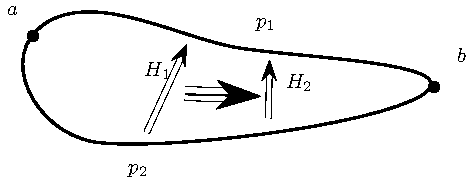
\includegraphics{path2}  
  \caption{Paths: $a$ and $b$ are points, $p_1$ and $p_2$ paths, $H_1$
  and $H_2$ homotopies.}
  \label{fig:paths}
\end{figure}
Indeed, that interpretation allows to explain all properties of
identity types.
\begin{itemize}
\item The equality $1_x$ is just the constant path 
  \[ \fonction{1_x}{[0,1]}{A}{t}{x} \]
\item The inverse $\inv \bullet$ is the function changing a path $f$ into
  \[ \fonction{g}{[0,1]}{A}{t}{f(1-t)} \]
\item The concatenation $\concat\bullet\bullet$ is the function
  changing paths $f$ and $g$ into
\[ \fonction{h}{[0,1]}{A}{t}%
  { \left\{
    \begin{array}{ll}
      f\left(2t\right) &\text{if } t\in[0,\nicefrac12] \\
      g\left(2t-1\right) &\text{if } t\in [\nicefrac12,1] 
    \end{array}
  \right.}
\]
\item A path between paths $f$ and $g$ between points $x$ and $y$ is a
  continuous function
  \[ 
    \fonction{H}{[0,1]²}{A}{(u,v)}{H(u,v)}
  \]
  such that $H(t,0) = f(t)$, $H(t,1) = g(t)$, $H(0,s)=x$ and
  $H(1,s)=y$. 
  A homotopy is then a continuous deformation of $f$ into $g$, fixing
  the ending points $x$ and $y$.
\end{itemize}

The table~\ref{fig:3pw} summarize the three points of view (type
theoretic, groupoidal, homotopy theoretic). In the rest of the thesis,
we will use any of the following name (\eg{} we will talk about
``points of a type'', ``path betwenn inhabitants'', \etc{}).

\begin{table}[h]
  \centering
  \begin{tabular}{|l|l|l|}
    \hline
    Type theory & Homotopy theory & $\omega$-groupoid \\
    \hline \hline
    Type & Topological space & $\omega$-groupoid \\
    \hline
    Inhabitant & Point & Object \\
    \hline
    Equality & Path & Morphism \\
    \hline
    $\idpath_x$ & Constant path & Identity morphism \\
    \hline
    $\inv\bullet$ & Inverse path & Inverse morphism \\
    \hline
    $\concat\bullet\bullet$ & Concatenation of paths & Composition of
                                                       morphisms \\
    \hline
    Equality between equalities & Homotopy & $2$-morphism\\
    \hline
  \end{tabular}
  \caption{Three points of view about HoTT}
  \label{fig:3pw}
\end{table}


What homotopy theorists love to do is to compute fundamental groups
(\ie{} the group of paths between two points) of
different spaces~(\cite{wangxu}\todo[fancyline]{These references
  were added without even opening them. Maybe a check would be good}
\cite{hutchings2011introduction}). We
can then categorized spaces with the level at which their homotopy
groups become trivial. Voevodsky has realized that this notion admits
a compact inductive definition internal to type theory, given by
\begin{defi}[Truncated types]
  $\IsType n$ is defined by induction on $n\geqslant -2$:
  \begin{itemize}
  \item $\IsType {(-2)}(X)$ if $X$ is a contractible type, \ie{} $X$
    is inhabited by $c:X$, and every other point in $X$ is connected to $c$.
  \item $\IsType {(n+1)}(X) \defeq \prod_{x,y:X} \IsType n (x=y).$
  \end{itemize}
  Then, $\Type_n \defeq \sum_{X:\Type} \IsType
  n(X)$\nomenclature{$\Type_n$}{Type of $n$-truncated types}.
\end{defi}

For the first values of $n$, there are different names:
$(-2)$-truncated types are called {\em contractible types},
$(-1)$-truncated types are called {\em h-propositions},
$0$-truncated types are called {\em h-sets}. Following this,
$\IsType{(-2)}$ is just $\Contr$, $\IsType{(-1)}$ is just $\IsHProp$
and $\Type_{-1}$ is $\HProp$, and $\IsType0$ is just $\IsHSet$ and
$\Type_0$ is $\HSet$. An explanation of this terminology might be
helpful. Contractible types are types, inhabited by a center $c$, with
paths between any point and $c$. A kind of magic thing about
contractible types is the lemma
\begin{lem}
  If $A:\Type$ is contractible, then for any $x,y:A$, the type $x=y$
  is contractible.
\end{lem}
Inductively, it means that paths types of any level over a contractible
type is contractible. It can be seen as the fact that a contractible
type contains only one point $c$, for which there is only one path
$c=c$, \etc{} The canonical example of contractible type is $\one$,
and actually, any contractible type is equivalent to $\one$.
Then, h-propositions are types where any two points are connected by a
path. The only difference with contractible types is that we allow the
type not to be inhabited. H-propositions are then proof-irrelevant
types, in the sense that under the propositions-as-types principle,
any points $x$ and $y$ in an $\HProp$ are equal, with a unique
equality, which is thus irrelevant.
\begin{lem}[Example of h-propositions]
  The following types are h-propositions:
  \begin{itemize}
  \item $\zero,\one$
  \item $\IsEquiv(f)$ for any $A,B:\Type$ and $f:A\to B$.
  \item $\IsType n(A)$ for any type $A:\Type$ and truncation index $n$.
  \end{itemize}
\end{lem}
Now, by definition, h-sets are types for which identity types are in
$\HProp$. The world of h-sets can thus be seen as the ``usual
mathematical'' world, as it satisfies proof-irrelevance.

The $n$-truncated types are stable under a lot of operations, as:
\begin{lem}
  Let $n\geqslant -2$ be a truncation index. Then
  \begin{itemize}
  \item If $A:\Type_n$ and $x,y:A$, then $\IsType n (x=y)$.
  \item If $A:\Type_n$ and $B:A\to\Type_n$, then $\IsType n
    \left(\sumD x A {B\, a}\right)$.
  \item If $A:\Type$ and $B:A\to\Type_n$, then $\IsType n \left(\prodD
      x A {B\, a}\right)$. Note that the source type needs not to be truncated.
  \item If $X:\Type_n$, $Y:\Type$ and $X\simeq Y$, then $\IsType
    n(Y)$.
  \item If $X:\Type_n$, then $\IsType{(n+1)}(X)$.
  \item We have $\IsType{(n+1)}{\Type_n}$.
  \end{itemize}
\end{lem}

\begin{rmq}
Some types are not $n$-truncated for any
$n$~\cite[Example 8.8.6]{hottbook} ; it is highly suspected for
example that the sphere $\mathbb S^2$ is one of
these $\infty$-truncated types (it is at least true in homotopy theory).  
\end{rmq}


This stratification of types induces a stratification of functions. A
function $f:A\to B$ is said to be $n$-truncated if all its homotopy
fibers $\fib f b$ are $n$-truncated. If $B:\Type$, a type $A$ together
with a $n$-truncated map $f:A\to B$ will be called a $n$-subobject of $B$.

As in~\cite{sets_in_hott}, we can define a sequence of subobject
classifiers, namely, $\Type_n$ classifies $n$-subobjects of a type
$B$, in the sens that there is an equivalence
\[\Xi : \sumD A \Type {\sumD f {A\to B} {\prodD b B
{\IsType n\
\fib{f}{b}}}} \xrightarrow{\sim} 
 (B \to \Type_n)\]
such that the diagram
\[
\xymatrix{
  A \ar[r]^{\hspace{-1em} t_f} \ar[d]_f & \Type_n^\bullet \ar[d]^{\pi_1}\\
  B \ar[r]_{\hspace{-1em} \chi_f} & \Type_n
}
\]
is a pullback for any $f$ with
 $n$-truncated homotopy fibers where $\Type_n^\bullet \defeq
 \sumD A \Type A$ is the universe of pointed
$n$-truncated types and 
\[ t_f = \lambda a,~(\fib{f}{f(a)},(a,\mathrm{idpath})). \]

We will use the equivalence $\Xi$ to define $n$-subobjects of a type
$B$ either as a $n$-truncated map $A\to B$, either as a characteristic
map $\chi:B\to\Type_n$.
\subsection{Truncations}
\label{ssec:trunc}

We present here a way to change any type into a $n$-truncated type, using
truncations. The interested reader can read Nicolai Kraus' PhD
thesis~\cite{phdkraus} consecrated to truncation levels in HoTT.

Let $n\geqslant -1$ be a truncation index. The $n$-truncation of a
type $A$ is the
higher inductive type $\|A\|_n$ \nomenclature{$\Vert\cdot\Vert$}{$n$-truncation of types}
 generated by
\[
  \left|
    \begin{array}{lll}
      \tr_n &:& A \to \|A\|_n \\
      \alpha_{\tr}^n &:& \IsType n (\|A\|_n)
    \end{array}
  \right.
\]
If $a:A$, $\tr_n(a)$ will be noted $|a|_n$.
The elimination principles are:
\begin{lem}[Elimination principle of truncations]\label{lem:trunc_elim}
  Let $A:\Type$ and $n\geqslant -1$ be a truncation index.
  \begin{itemize}
  \item If $P:\Type$ such that $\IsType n(P)$ and $f:A \to P$, then
    there is a map
    \[|f|_n : \|A\|_n \to P\]
    such that for all $a:A$, $|f|_n(|a|_n) \equiv f(a)$.
  \item If $P:\|A\|_n \to \Type$ such that $\prodD x {\|A\|_n}
    {\IsType n (P\, x)}$ and $f:\prodD a A {P(|a|_n)}$, then there is
    a dependent map
    \[|f|_n : \prodD x {\|A\|_n} {P\, x}\]
    such that for all $a:A$, $|f|_n(|a|_n) \equiv f(a)$.
  \end{itemize}
\end{lem}
\nomenclature{$\vert\cdot\vert_n$}{$n$-truncation of terms or arrows}
Basically, this induction principle says that $\|A\|_n$ has contains
as much data about $A$ than $A$ itself, but it can only be used to
define a $n$-truncated type. It can be expressed as the following
universal property:
\begin{lem}[Universal property of truncations]
  Let $A:\Type$ and $P:\Type_n$. Then the map
\todo[fancyline]{Check post or pre}
\[
  \fonction{\precompose_{\tr_n}}{A\to P}{\|A\|_n \to P}{f}{f \circ \tr_n}
\]
is an equivalence.
\end{lem}
We will see in chapter~\ref{chap:modalities} that all $(\IsType
n,\|\bullet\|_n)$ define {\em modalities}. In particular, every
truncation index $n$ yields a factorization system:

\begin{prop}
  Let $n\geqslant -1$ a truncation index. Then any map $f:A\to B$ can
  be factored as a $n$-connected map followed by a $n$-truncated map,
  where a map is $n$-connected if for all $b:B$, $\|\fib f b\|_n$ is contractible.
\end{prop}

In the rest of this thesis, we will only use this result with
$n=-1$. In that case, $(-1)$-truncated functions are called {\em
  embeddings}, and $(-1)$-connected functions are called {\em
  surjections}. The factorization of a map $f:A\to B$ is given by
\[
  \xymatrix{
    A \ar[rr]^f \ar[rd]^{\widetilde f} && B \\
    & \im(f)  \ar[ru]^{\pi_1} &
  }
\]
\begin{align*}
  \im(f) &\defeq \sumD b B {\left\| \sumD a A {f\, a = b}
  \right\|_{-1}} \\
  \widetilde f &\defeq \lambda a:A,\, \left(f\, a,\left|(a,1_b)\right|_{-1}\right)
\end{align*}

%%% Local Variables:
%%% mode: latex
%%% TeX-master: "main"
%%% End:

\chapter{Higher modalities}
\label{chap:modalities}

As said in the introduction, the main purpose of our work is to build,
from a model $\mathfrak M$ of homotopy type theory, another model
$\mathfrak M'$ satisfying new principles. Of course, $\mathfrak M'$
should be describable {\em inside} $\mathfrak M$. In set theory, it
corresponds to building {\em inner models} (\cite{kunen}).%
%
In type theory, it can be rephrased in terms of left-exact modalities:
it consists of an operator $\modal$ on types such that for any type
$A$, $\modal A$ satisfies a desired property. If the operator has a
``good'' behaviour, then it is a modality, and the universe of all
types satisfying the chosen property forms a new model of homotopy
type theory.

\section{Modalities}
\label{sec:modalities}

\begin{defi}
  \label{def:modality}
  A left exact modality is the data of
  \begin{enumerate}[(i)]
  \item A predicate $P:\Type \to \HProp$
  \item For every type $A$, a type
    $\modal A$ such that $P(\modal A)$
  \item For every type $A$, a map $\eta_A:A \to
    \modal A$
  \end{enumerate}
  such that
  \begin{enumerate}[(i)]
    \setcounter{enumi}{3}
  \item For every types $A$ and $B$, if $P(B)$ then
    \[ \left\{
        \begin{array}{rcl}
          (\modal A \to B) & \to & (A \to B) \\
          f & \mapsto & f \circ \eta_A
        \end{array} \right. \] %
    is an equivalence.
  \item for any $A:\Type$ and $B:A \to \Type$ such that $P(A)$
    and $\prod_{x:A} P(B x)$, then $P\left( \sum_{x:A} B(x)\right)$
  \item for any $A:\Type$ and $x,y:A$, if $\modal A$ is
    contractible, then $\modal (x=y)$ is contractible.
  \end{enumerate}
  Conditions (i) to (iv) define a {\em reflective subuniverse}, (i) to
  (v) a {\em modality}.
\end{defi}

\section{Examples of modalities}
\label{sec:modalities-examples}

\subsection{The identity modality}
\label{ssec:id_mod}

Let us begin with the most simple modality one can imagine: the one
doing nothing. We can define it by letting $\modal A \defeq A$ for any type
$A$, and $\eta_A \defeq \idmap$. Obviously, the desired computation
rules are satisfied, so that the identity modality is indeed a
left-exact modality.

It might sound useless to consider such a modality, but it can be
precious when looking for properties of modalities: if it does not
hold for the identity modality, it cannot hold for an abstract one.


\subsection{Truncations}
\label{ssec:truncations}

The first class of non-trivial examples might be the {\em truncations}
modalities.

\subsection{Double negation modality}
\label{ssec:notnot}

The double negation modality $\modal A \defeq \lnot\lnot A$ is a
modality. Unfortunately, it appears that every type is collapsed to an
$\HProp$, thus it cannot be used as-is. The main purpose of this
thesis, in particular chapter~\ref{chap:sheaf} is to extend this
modality into a better one.

\section{New type theories}
\label{sec:translation}

\section{Truncated modalities}
\label{sec:trunc_modalities}


\chapter{Colimits}
\label{chap:colim}

\epigraph{A comathematician is a device turning cotheorems into
  ffee.}{Mathematical folklore}

As seen in chapter~\ref{chap:hott}, adding sigma-types to type theory
results in adding limits over graphs in the underlying category, and
adding higher inductives typves results in adding colimits over
graphs. If limits has been extensively studied in~\cite{lumsdaine},
theory of colimits was not completely treated.

The following is conjoint work with Simon Boulier and Nicolas
Tabareau, helped by precious discussions with Egbert Rijke.
The sections~\ref{sec:colim} and~\ref{sec:floris} are extended version
of the blog post~\cite{boulier}.

\section{Colimits over graphs}
\label{sec:colim}

As colimits are just dual to limits, it seems that it would be very
easy to translate the work on limits to colimits. Althought, even if
it might be because we are more habituated to manipulate sigma-types
than higher inductive types, it seems way harder.

\subsection{Definitions}
\label{ssec:colim:defi}

Let's recall the definitions of graphs and diagrams over graphs,
introduced in~\cite{lumsdaine}.

\begin{defi}[Graph]\label{defi:graph}
  A {\em graph} $G$ is the data of
  \begin{itemize}
  \item a type $G_0$ of vertices ;
  \item for any $i,j:G_0$, a type $G_1(i,j)$ of edges.
  \end{itemize}
\end{defi}

\begin{defi}[Diagram]\label{defi:diagram}
  A {\em diagram} $D$ over a graph $G$ is the data of
  \begin{itemize}
  \item for any $i:G_0$, a type $D_0(i)$ ;
  \item for any $i,j:G_0$ and all $\phi : G_1(i,j)$, a map $D_1(\phi)
    : D_0(i) \to D_0(j)$
  \end{itemize}
\end{defi}

When the context is clear, $G_0$ will be simply denoted $G$,
$G_1(i,j)$ will be noted $G(i,j)$, $D_0(i)$
will be noted $D(i)$ or $D_i$, and $D_1(\phi)$ will be noted
$D_{i,j}(\phi)$ or simply $D(\phi)$ ($i$ and $j$ can be inferred from
$\phi$).

\begin{exms}
  \item One can consider the following graph, namely the graph of
    (co)equalizers
    \[ \xymatrix{\bullet \ar@<-.5ex>[r] \ar@<.5ex>[r] & \bullet} \]
    Here, $G_0 = \two$, $G_1(\True,\False) = \two$ and other
    $G_1(i,j)$ are empty.

    A diagram over this graph consists of two types $A$ and $B$, and
    two maps $f,g:A \to B$, producing the diagram
    \[ \xymatrix{A \ar@<-.5ex>[r]_g \ar@<.5ex>[r]^f & B} \]
  \item The graph of the mapping telescope is 
    \[ \xymatrix{ \bullet \ar[r] &\bullet \ar[r] &\cdots} \]
    In other words, $G_0=\N$ and $G_1(i,i+1) = \one$.

    A diagram over the mapping telescope is a sequence of types $P:\N
    \to \Type$ together with arrows $f_n:P_n \to P_{n+1}$:
    \[ \xymatrix{ P_0 \ar[r]^{f_0} & P_1 \ar[r]^{f_1} & \cdots} \]
\end{exms}

What we would like now would be to define the colimits of these
diagrams over graphs, that would satisfy type theoretic versions of
usual properties: it should make the diagram commute, and be universal
with respect to this property.
From now on, let $G$ be a graph and $D$ a diagram over this graph.

The commutation of the diagram is easy: the colimit should be the tip
of a cocone.

\begin{defi}[Cocone]\label{defi:cocone}
  Let $Q$ be a type. A cocone over $D$ intro $Q$ is the data of arrows
  $q_i:D_i \to Q$, and for any $i,j:G$ and $g:G(i,j)$, an homotopy 
  $q_j \circ D(g) \homot q_i$.
\end{defi}

If $Q$ and $Q'$ are type with an arrow $f:Q\to Q'$, and if $C$ is a
cocone over $D$ into $Q$, one can easily build a cocone on $D$ into
$Q'$ by postcomposing all maps of the cocone by $f$, giving a map
\newcommand{\postcomposecocone}{\mathrm{postcompose}_{\mathrm{cocone}}}
\[\postcomposecocone : \cocone_D(Q) \to (Q':\Type) \to (Q \to Q') \to \cocone_D(Q') \]
The other way around (from a cocone into $Q'$, give a map $Q\to Q'$)
is exactly the second condition we seek:

\begin{defi}[Universality of a cocone]
  Let $Q$ be a type, and $C$ be a cocone over $D$ into $Q$. $C$ is
  said universal if for any type $Q'$, $\postcomposecocone(C,Q')$ is
  an equivalence.
\end{defi}

We can finally define what it means for $Q$ to be a colimit of $D$.

\begin{defi}[Colimit]\label{defi:colimit}
  A type $Q$ is said to be a colimit of $D$ if there is a cocone $C$
  over $D$ into $Q$, which is universal.
\end{defi}

\begin{exm}
  Let $A$, $B$ be types and $f,g:A\to B$.
  Let $Q$ be the HIT generated by
  $\left|
  \begin{array}{lll}
    q & : & B \to Q \\
    \alpha & : & q \circ f \homot q \circ g
  \end{array} \right. .$
Then $Q$ is a colimit of the coequalizer diagram associated to
$A,B,f,g$. We say that $Q$ is a coequalizer of $f$ and $g$.
\end{exm}

Note that for any diagram $D$, one can build a free colimit of $D$,
namely the higher inductive type $\colim(D)$ generated by
\[ 
  \left|
    \begin{array}{lll}
      \colim & : & \prodD i G {D_i \to \colim(D)} \\
      \alpha_\colim & : & \prodD {i j} G {\prodD g {G(i,j)} {\prodD x
                          {D_i} {\colim_j \circ D(g) \homot \colim_i}}}
    \end{array} \right.
\]


\todo[inline]{Finish colimits}
\subsection{Properties of colimits}
\label{ssec:prop_colim}

\subsection{Truncated colimits}
\label{ssec:trunc_colim}

As said in\todo[fancyline]{Insert here a relevent ref}, we now give a
truncated version of colimits. 
Colimits actually behave well with respect to truncations. Indeed, if $D$ is a
diagram and $P$ a colimit of $D$, then $\|P\|_n$ is the $n$-colimit
of the $n$-truncated diagram $\|D\|_n$. Let's make it more precise.

\begin{defi}[Truncation of a diagram]
  Let $D$ be a diagram over a graph $G$, and $n$ a truncation index.
  Then the diagram $\|D\|_n$ is the diagram over $G$ defined by
  \begin{itemize}
  \item $(\|D\|_n)_0(i) \defeq \|D_0(i)\|_n:\Type_n$
  \item $(\|D\|_n)_1(\phi) \defeq |D_1(\phi)|_n : \|D_0(i)\|_n \to \|D_0(j)\|_n$
  \end{itemize}
\end{defi}

\begin{defi}
  Let $D$ be a diagram over a graph $G$, $P$ be a type, and $C$ a
  cocone over $D$ into $P$. $C$ is said $n$-universal if for any
  $Q:\Type_n$, $\postcompose_{\mathrm{cocone}}(C,Q)$ is an
  equivalence.

  Then, $P$ is said to be a $n$-colimit of $D$ if there is a cocone
  $C$ over $D$ into $Q$ which is $n$-universal.
\end{defi}

We can now give the fundamental proposition linking colimit and
$n$-colimit.

\begin{prop}
  Let $D$ be a diagram, and $P:\Type$.
  Then, if $P$ is a colimit of $D$, $\|P\|_n$ is a $n$-colimit of $\|D\|_n$.
\end{prop}

The proof of this is really straightforward: a cocone over $D$ into
$P$ can be changed equivalently into a cocone over $\|D\|_n$ into $\|P\|_n$, using the
elimination principle~\ref{lem:trunc_elim} of truncations, and then
we can show that the following diagram commutes for any $X:\Type_n$
\[
  \xymatrix{
    \|P\|_n \to X \ar[r] \ar[d]^*[@]{\hbox to 0pt{\hss$\sim$\hss}} & \mathrm{cocone}(\|D\|_n,X) \\
    P \to X \ar[r]^\sim& \mathrm{cocone}(D,X) \ar[u]^*[@]{\hbox to 0pt{\hss$\sim$\hss}}
  }
\]

\begin{rmq}
This result does not hold for limits. If it were
true, then applying it to the following equalizer diagram
\[ \xymatrix{ A \ar@<-.5ex>[r]_{\lambda \_,\,y} \ar@<.5ex>[r]^f & B }\]
with $A,B:\Type$, $f:A\to B$ and $y:B$ would lead to an equivalence
\[ \left\| \sumD a A {f a = y} \right\|_{n} \simeq \sumD a {\|A\|_{n}}
  {|f|_{n}\, a = |y|_{n}}, \]
proving left-exactness of $n$-truncation.  
\end{rmq}

\subsection{Towards highly coherent colimits}
\label{ssec:high_colimit}

\section{Van Doorn's and Boulier's constructions}
\label{sec:floris}

\begin{prop}\label{prop:cech}
  
\end{prop}

\section{Towards groupoid objects}
\label{sec:groupoid}
\chapter{Sheaves in homotopy type theory}
\label{chap:sheaf}
\epigraph{Reductio ad absurdum, which Euclid loved so much, is one of
  a mathematician's finest weapons. It is a far finer gambit than any
  chess gambit: a chess player may offer the sacrifice of a pawn or
  even a piece, but a mathematician offers the game}{G.H. Hardy}

Section~\ref{sec:sheaf_topos} briefly recalls the topos-theoretic
version of Lawvere-Tierney sheaves theory, and
section~\ref{sec:sheaf_hott} presents the main result of this thesis:
the construction of the sheafification modality in homotopy type
theory. Section~\ref{sec:forcing} tries to link our construction
with forcing in type theory.

\section{Sheaves in topoi}
\label{sec:sheaf_topos}

In this section, we will rather work in an arbitrary topos rather in type theory. The next section will present a
generalisation of the results presented here.

Let us fix for the whole section a topos $\mathcal E$, with subobject
classifier $\Omega$. A {\em Lawvere-Tierney topology} on $\mathcal E$
is a way to modify slightly truth values of $\mathcal E$. It allows to
speak about {\em locally true} things instead of {\em true} things.

\begin{defi}[Lawvere-Tierney topology~\cite{maclanemoerdijk}]\label{defi:LT}
  A Lawvere-Tierney topology is an endomorphism $j:\Omega \to \Omega$
  preserving $\True$ ($j \ \True = \True$), idempotent ($j\circ j =
  j$) and commuting with products ($j \circ \wedge = \wedge \circ (j,j)$).
\end{defi}

A classical example of Lawvere-Tierney topology is given by double
negation. Other examples are given by Grothedieck topologies, in the
sense
\begin{thm}[{\cite[V.1.2]{maclanemoerdijk}}]
  Every Grothendieck topology $J$ on a small category $\mathbf C$ determines a
  Lawvere-Tierney topology $j$ on the presheaf topos
  $\mathbf{Sets}^{\mathbf C^{\mathbf{op}}}$.
\end{thm}

Any Lawvere-Tierney topology $j$ on $\mathcal E$ induces a closure operator
$A \mapsto \closure{A}$ on subobjects. If we see a subobject $A$ of $E$
as a characteristic function $\Char{A}$, the closure $\closure{A}$
corresponds to the subobject of $E$ whose characteristic function is 
%
\[
\Char{\closure{A}} = j \circ \Char{A}.
\]%
%
A subobject $A$ of $E$ is said to
be dense when $\closure{A} = E$.

Then, we are interested in objects of $\mathcal E$ for which it is
impossible to make a distinction between objects and their dense
subobjects, \ie{} for which ``true'' and ``locally true''
coincide. Such objects are called {\em sheaves}, and are defined as

\begin{defi}[Sheaves{\cite[V.2]{maclanemoerdijk}}]
  On object $F$ of $\mathcal E$ is a sheaf (or $j$-sheaf) if for every
  dense monomorphism $m: A \hookrightarrow E$ in $\mathcal E$, the
  canonical map $\Hom{\mathcal E}(E,F) \rightarrow \Hom{\mathcal E}(A,F)$ is an
isomorphism.
\end{defi}

One can show that $\Sh{\mathcal E}$, the full sub-category of
$\mathcal E$ given by
sheaves, is again a topos, with classifying object
%
\[
\Omega_j = \{ P \in \Omega \ | \ j P  = P \}.
\]

Lawvere-Tierney sheafification is a way to build a left adjoint $\mathbf{a}_j$ to the
inclusion $\mathcal E \hookrightarrow \Sh(\mathcal E)$, exhibiting
$\Sh(\mathcal E)$ as a reflective subcategory of $\mathcal E$. In
particular, that implies that logical principles valid in $\mathcal E$
are still valid in $\Sh(\mathcal E)$.

For any object $E$ of $\mathcal E$, $\mathbf{a}_j(E)$ is defined as in
the following diagram
\[
  \xymatrix{ 
    E \ar[rr]^{\{\cdot\}_E} \ar@{->>}[d]_{\theta_E} && \Omega^E \ar[d]^{j^E}\\
    E' \ar@{^{(}->}[rr] \ar[dr]_{\text{closure}} && \Omega_j^E \\
    & \mathbf{a}_j(E) \ar[ur]&
  }
\]

The proof that $\mathbf a_j$ defines a left adjoint to the inclusion
can be found in~\cite{maclanemoerdijk}.

One classical example of use of sheafification is the construction,
from any topos, of a boolean topos negating the continuum
hypothesis. More precisely:

\begin{thm}[Negation of CH~{\cite[VI.2.1]{maclanemoerdijk}}]
  There exists a Boolean topos satisfying the axiom of choice, in
  which the continuum hypothesis fails.
\end{thm}

The proof actually follows almost exactly the famous proof of the
construction by Paul Cohen of a model of ZFC negating the continuum
hypothesis~\cite{cohen1966}. Together with the model of constructible
sets $\mathfrak L$ by Kurt Gödel~\cite{godel40}, it proves that CH is
independent of ZFC, solving first Hilbert's problem.


\section{Sheaves in homotopy type theory}
\label{sec:sheaf_hott}

The idea of this section is to consider sheafification in topoi as
only the first step towards sheafification in type theory. 
We note that axioms for a Lawvere-Tierney topology on the subobject
classifier $\Omega$ of a topos are very close to
those of a modality on $\Omega$. We will extensively use this idea,
applying it to every subobject classifier $\Type_n$ we described
in~\ref{sec:hott}. The subobject
classifier $\Omega$ of a topos is seen as the {\em truth values} of the
topos, which corresponds to the type $\HProp$ in our setting ; the
topos is considered proof irrelevant, corresponding to our
$\HSet$. Sheafification in topoi is thus a way, when translated to the
setting of homotopy type theory, to build, from a left-exact modality on
$\HProp$, a left-exact modality on $\HSet$. Our hope in this section
is to iterate this construction by applying it to the subobject
classifier $\HSet$ equipped with a left-exact modality, to build a new
left-exact modality on $\Type_1$, and so on. 

The first thing we can
note is that such a construction will not allow to reach every type:
it is known that there exists types with no finite truncation
level~\cite[Example 8.8.6]{hottbook}. Even worse, some types are not
even the limit of its successive truncations, even in a hypercomplete
setting~\cite{morelvv}. It suggests that defining a sheafification
functor for all truncated types won't give (at least easily) a
sheafification functor on whole $\Type$.
Another issue that can be pointed is the complexity of proofs. If, in
a topos-theoretic setting, everything is proof-irrelevant, it won't be
the case for higher settings, forcing us to prove results that were
previously true on the nose. This will oblige us to write long and
technical proofs of coherence, and more deeply, to modify completely
some lemmas, such as Proposition~\cite[IV.7.8]{maclanemoerdijk},
stating that epimorphisms are coequalizers of their kernel pair.

The main idea is thus to follow as closely as possible the
topos-theoretic construction, and change as few times as possible to
make it work in our higher setting.

Note that the principles we want to add are added directly from the
$\HProp$ level, the extension to all truncated types is automatic. The
choice of the left-exact modality on $\HProp$ is thus crucial. For the
rest of the section, we fix one, note $\modal_{-1}$. The reader can
think of the double negation $\modal_{\lnot\lnot}$ defined
in~\ref{ssec:notnot}. We will define, by induction on the truncation
level, left-exact modalities on all $\Type_n$, as in the following
theorem.

\begin{thm}\label{thm:main}
  The sequence defined by induction by
  \[ \begin{array}{l}
   \modal : \forall \ (n : nat), \ \Type_n \to \Type_n 
   \\
    \modal_{-1\phantom{n}}(T) \defeq \mathop{j} T \\

      \displaystyle{\modal_{n+1}(T)} \defeq  
      \displaystyle{\sum_{u:T \to \Type_n^\modal} \!\!\!\!\modal_{-1} 
      \left\|
      \sum_{a:T} u= (\lambda t,~\modal_n (a=t))
      \right\|}
    \end{array}
\]
defines a sequence of left-exact modalities, coherent with each others
in the sense that the following diagram commutes for any $P:\Type_n$,
where $\hat P$ is $P$ seen as an inhabitant of $\Type_{n+1}$.
\[ \xymatrix{
    P \ar@{->}^{\sim}[r] \ar[d]_{\eta_{n}} & \widehat P \ar[d]^{\eta_{n+1}} \\
    \modal_{n} P \ar@{->}^{\sim}[r] & \modal_{n+1} \widehat P 
  } \]
\end{thm}

\subsection{Sheaf theory}
\label{ssec:sheaves}

Let $n$ be a truncation index greater that $-1$, and $\modal_n$ be the
left-exact modality given by our induction hypothesis. As in the
topos-theoretic setting, we will define what it means for a type to be
a $n$-sheaf (or just ``sheaf'' if the context is clear), and consider
the reflective subuniverses of these sheaves ; the reflector will
exactly be the sheafification functor.
The main issue to give the ``good'' definition is the choice of the
subobject classifier in which dense subobjects will be chosen: two
choices appears, $\HProp$ and $\Type_n$ ; we will actually use
both. What guided our choice is the crucial property that the type of
all $n$-sheaves has to be a $(n+1)$-sheaf.

From the modality $\modal_n$, one can build a {\em closure operator}.

\begin{defi}
  Let $E$ be a type. 
  \begin{itemize}

  \item The {\em closure} of a subobject of $E$ with
  n-truncated homotopy fibers (or $n$-subobject of $E$, for short),
  classified by $\chi : E \to \Type_n$, is the subobject of $E$
  classified by $\modal_n \circ \chi$.

  
\item An $n$-subobject of $E$ classified by $\chi$ is said to be {\em
    closed in $E$} if it is equal to its closure, \ie{} if
  $\chi = \modal_n \circ \chi$.

  
\item An $n$-subobject of $E$ classified by $\chi$ is said to be {\em
    dense in $E$} if its closure is $E$, \ie{} if 
  $\modal_n \circ \chi = \lambda e, \one$ 
  \end{itemize}
\end{defi}


Topos-theoretic sheaves are characterized by a property of existence
and uniqueness, which will be translated, as usual, into a proof that
a certain function is an equivalence.

\begin{defi}[Restriction]
  Let $E,F:\Type$ and $\chi:E\to\Type$. We define the {\em
    restriction map} $\Phi_E^\chi$ as follows
  \[
    \fonction{\Phi_E^\chi}{E\to F}{\sumD e E {\chi e} \to F}{f}{f\circ \pi_1}.
  \]
\end{defi}

Here, we need to distinguish between
dense $(-1)$-subobjects, that will be used in the definition of
sheaves, and dense $n$-subobjects, that will be used in the definition
of separated types. 

\begin{defi}[Separated Type]
  A type $F$ in $\Type_{n+1}$ is {\em separated} if for any type $E$, and
  all dense $n$-subobject of $E$ classified by $\chi$,
  $\Phi_E^\chi$ is an embedding.
\end{defi}

With topos theory point of view, it means that given a map $\sum_{e:E}
\chi\, e \to F$,
if there is an extension $\tilde f:E\to F$, then it is unique, as in
 \[ \xymatrix{
    \sumD e E {\chi e} \ar[r]^-f \ar[d]_{\pi_1} & F \\
    E \ar@{-->}[ru]_{!}&
  }\]
\begin{defi}[Sheaf]
  A type $F$ of $\Type_{n+1}$ is a {\em $(n+1)$-sheaf} if it is
  separated, and for any type $E$ and all dense $(-1)$-subobject of
  $E$ classified by $\chi$, $\Phi_E^\chi$ is an
  equivalence.
\end{defi}

In topos-theoretic words, it means that given a map $f : \sum_{e:E}
\chi\, e\to F$, one can
extend it uniquely to $\tilde f:E \to F$, as in 
 \[ \xymatrix{
    \sumD e E {\chi e} \ar[r]^-f \ar[d]_{\pi_1} & F \\
    E \ar@{-->}[ru]_{\exists !}&
  }\]

Note that these definitions are almost the same as the ones
in~\cite{maclanemoerdijk}. The main difference is that {separated}
is defined for $n$-subobjects, while {sheaf} only for
$(-1)$-subobjects. It might seem bizarre to make such a distinction,
but the following proposition gives a better understanding of the situation.
\begin{prop}
  A type $F$ is $\Type_{n+1}$ is separated if, and only if all its
  path types are $n$-modal, ie
  \[ \prodD {x,y} F {\left( \modal_n(x=y) \right) = (x=y)}.\]
\end{prop}

A $(n+1)$-sheaf is hence just a type satisying the usual property of sheaves
(\ie{} existence of uniqueness of arrow extension from dense
$(-1)$-subobjects), with the condition that all its path types are
$n$-sheaves. It is a way to force the compatibility of the modalities we
are defining.


On can check that the property $\issep$ (resp. $\issheaf$) is $\HProp$:
given a $X:\Type_{n+1}$, there is only one way for it to be separated
(resp. a sheaf). In particular, when needed to prove equality between
two sheaves, it suffices to show the equality between the underlying
types.


As said earlier, these definitions allow us to prove the fundalemental
property that the type of all $n$-sheaves is itself a $(n+1)$-sheaf
(this can be viewed as an equivalent definition of left-exactness).

\begin{prop}\label{prop:sheaf-is-sheaf}
  $\Type_n^\modal$ is a $(n+1)$-sheaf.
\end{prop}

\begin{proof}
  We have two things to prove here : separation, and sheafness.
  \begin{itemize}
  \item Let $E:\Type$ and $\chi:E\to\Type$, dense in $E$. 
    Let $\phi_1,\phi_2:E \to
    \Type_n^\modal$, such that $\phi_1 \circ \pi_1 = \phi_2 \circ
    \pi_1$ and let $x:E$. We show $\phi_1(x) = \phi_2(x)$ using
    univalence.
    
    As $\chi$ is dense, we have a term $m_x : \modal_n(\chi\, x)$.
    But as $\phi_2(x)$ is modal, we can obtain a term $h_x : \chi\,
    x$. 
    As $\phi_1$ and $\phi_2$ are equal on $\sumD e E {\chi\, e}$, we
    have an arrow $\phi_1(x) \to \phi_2(x)$.
    The same method leads to an arrow $\phi_2 (x) \to \phi_1 (x)$, and
    one can
    prove that they are each other inverse.
  \item Now, we prove that $\Type_n^\modal$ is a sheaf. Let $E:\Type$ and
  $\chi:E \to \HProp$, dense in $E$. Let $f:\sum_{e:E} \chi\, e \to
  \Type_n^\modal$. We want to extend $f$ into a map $E \to \Type_n^\modal$.

  We define $g$ as $g(e) = \modal_n \left( \fib \phi {e} \right)$,
  where
  \[ \phi : \sum_{b:\sumD e E {\chi\, e}} (f\,
    b) \to E\]
  defined by $\phi(x) = (x_1)_1$.
  Using the following lemma, one can prove that the map $f\mapsto g$
  defines an inverse of $\Phi_E^\chi$.
  \begin{lem}
    Let $A,B,C:\Type_n$, $f:A\to B$ and $g:B\to C$.
    Then
    if all fibers of $f$ and $g$ are $n$-truncated, then
      \[\left( \prodD c C {\modal_n(\fib {g \circ f} c)}\right) \simeq
      \modal_n \left(  
        \sumD w {\fib g c} {\modal_n (\fib f {w_1})}
      \right).\]
  \end{lem}
  \begin{prooflem}
    This is just a modal counterpart of the property characterizing
    fibers of composition of function.
  \end{prooflem}
  \end{itemize}
\end{proof}

Another fundamental property on sheaves we will need is that the type of (dependent)
functions is a sheaf as soon as its codomain is a sheaf.

\begin{prop}\label{prop:sheaf-forall}
  If $A:\Type_{n+1}$ and $B:A \to \Type_{n+1}$ such that for any
  $a:A$, $(B~a)$ is a sheaf, then $\prodD a A {B\, a}$ is a sheaf.
\end{prop}
\begin{proof}
  Again, when proving equivalences, we will only define the maps. The
  proofs of section and retraction are technical, not really
  interesting, and present in the formalisation.
  \begin{itemize}
  \item {\em Separation:} Let $E:\Type$ and $\chi:E \to \Type_n$ dense
    in $E$. Let $\phi_1,\phi_2:E\to \prodD a A {B\, a}$ equal on
    $\sumD e E{\chi\, e}$ \ie{} such that $\phi_1\circ \pi_1 = \phi_2\circ
    \pi_1$.
    Then for any $a:A$, $(\lambda x:E,~\phi_1(x, a))$
    and $(\lambda x:E,~\phi_2(x,a))$
    coincide on $\sum_{e:E}(\chi\, e)$, and as $B\, a$ is separated,
    they coincide also on all $E$.
  \item {\em Sheaf:} Let $E:\Type$, $\chi:E\to \HProp$ dense in $E$ and
    $f:\sumD e E {\chi\, e}\to \prodD a A{B\,a}$. Let $a:A$ ; the
    map $(\lambda x,~f(x,a))$ is valued in the sheaf $B\, a$, so it
    can be extended to all $E$, allowing $f$ to be extended to all
    $E$.
  \end{itemize}
\end{proof}

\subsection{Sheafification}
\label{ssec:sheafification}

The sheafification process will be defined in two steps. The first
one will build, from any $T:\Type_{n+1}$, a separated object $\separated
T:\Type_{n+1}$ ; one can show that $\separated$ defines a modality on
$\Type_{n+1}$. The second step will build, from any separated type
$T:\Type_{n+1}$, a sheaf $\modal_{n+1}(T)$ ; one can show that
$\modal_{n+1}$ is indeed the left-exact modality we are searching.

Let $n$ be a fixed truncation index, and $\modal_n$ a left-exact
modality on $\Type_n$, compatible with $\modal_{-1}$ as in
\begin{cond}\label{cond:hprop}
  For any mere proposition $P$ (where $\widehat P$ is $P$ seen as a
  $\Type_n$),  $\modal_n \widehat P = \modal_{-1} P$ and the
  following coherence diagram commutes
  \[\xymatrix{
    P \ar@{->}^{\sim}[r] \ar[d]_{\eta_{-1}} & \widehat P \ar[d]^{\eta_n} \\
    \modal_{-1} P \ar@{->}^{\sim}[r] & \modal_n \widehat P 
  }\]
\end{cond}

\subsubsection{From types to separated types}
\label{sssec:type_to_sep}


Let $T : \Type_{n+1}$. We define $\separated T$ as the image of
$\modal_n^T \circ \{\cdot\}_T$, as in
\[\xymatrix{
    T \ar[r]^{\{\cdot\}_T} \ar[d]_{\mu_T} & \left(\Type_n\right)^T \ar[d]^{\modal_n^T} \\
  \separated T \ar[r]& \left( \Type_n^\modal \right)^T
}, \]%
where $\{\cdot\}_T$ is the singleton map $\lambda (t:T),~\lambda
(t':T),~t=t'$. 
%
$\separated T$ can be given explicitly by
%
\begin{align*}
\separated T &\defeq \im (\lambda~t:T,~\lambda~ t',~ \modal_n (t = t')) \\
          &\defeq \sumD u{T \to \Type_n^\modal} {\left\| \sumD a A
            {(\lambda t,~\modal_n (a=t)) = u}\right\|}.
\end{align*}
%
This corresponds to the free separated object used in the topos-theoretic construction, but using $\Type_n^\modal$ instead of the
$j$-subobject classifier $\Omega_j$.
%
\begin{prop}
  For any $T:\Type_{n+1}$, $\separated T$ is separated.  
\end{prop}

\begin{proof}
We use the following lemma:
\begin{lem}\label{lem:embed-sep}
  A $(n+1)$-truncated type $T$ with an embedding $f : T \to U$
  into a separated $(n+1)$-truncated type $U$ is itself separated.
\end{lem}
\begin{prooflem}
  Let $E:\Type$ and $\chi:E\to\Type_n$ dense in $E$. Let
  $\phi_1,\phi_2:\sumD e E {\chi\, e} \to T$ such that $\phi_1 \circ
  \pi_1 \homot \phi_2 \circ \pi_1$. Post\todo[fancyline]{Post
    or Pre?}composing by $f$ yields an homotopy $f \circ \phi_1 \circ
  \pi_1 \homot f \circ \phi_2 \circ \pi_1$. As $f\circ\phi_1,f\circ
  \phi_2 : \sumD e E {\chi\, e} \to U$, and $U$ is separated, we can
  deduce $f \circ \phi_1 \homot f \circ \phi_2$. As $f$ is an
  embedding, $\phi_1 \homot \phi_2$.
\end{prooflem}
As $\separated T$ embeds in $\left( \Type_n^\modal \right)^T$, we only
have to show that the latter is separated. But it is the case because
$\Type_n^\modal$ is a sheaf (by Proposition~\ref{prop:sheaf-is-sheaf})
and a function type is a sheaf as soon
as its codomain is a sheaf (by Proposition~\ref{prop:sheaf-forall}).
\end{proof}

We will now show that $\separated$ defines a modality, with unit map
$\mu$. The left-exactness of $\modal_{n+1}$ will come from the second
part of the process.
The first thing to show that $\separated T$
is universal among separated type below $T$. 
In the topos-theoretic sheafification, it comes easily from the fact
that epimorphims are coequalizers of their kernel pairs. As it is not
true anymore in our setting, we will use its generalization,
proposition~\ref{prop:cech}.%
%
Here is a sketch of the proof:
as $\mu_T$ is a surjection (it is defined by the surjection-embedding
factorization), $\separated T$ is the colimit of its iterated kernel
pair. Hence, for any type $Q$ defining a cocone on $\KP(\mu_T)$, there
is a unique arrow $\separated T\to Q$. What remains to show is any
separated type $Q$ defines a cocone on $\KP(\mu_T)$ ; we will actually
show that any separated type $Q$ defines a cocone on
$\|\KP(\mu_T)\|_{n+1}$, which is enough. We do it by
defining another diagram $\mathring T$, equivalent to $\|\KP(\mu_T)\|_{n+1}$, for
which it is easy to define a cocone into any separated type $Q$.


This comes from the
following construction which connects $\separated T$ to the colimit of
the iterated kernel pair of $\mu_T$.

\begin{defi}
  Let $X:\Type$. Let $\mathring T_X$ be the higher inductive type
  generated by
  \begin{itemize}
  \item $\mathring t:~\|X\|_{n+1} \to \mathring T_X$
  \item $\mathring \alpha:~\forall a\, b:\|X\|_{n+1},~\modal (a=b) \to
    \mathring t(a) = \mathring t(b)$
  \item $\mathring \alpha_1:~\forall a:\|X\|_{n+1},~
    \mathring \alpha(a , a, \eta_{a=a} 1) = 1$
  \end{itemize}

  We view $\mathring T$ as the coequalizer of
  \[
    \xymatrix{\displaystyle{\sumD {a,b}{\|X\|_{n+1}} {\modal (a=b)}} \ar@<-.5ex>[r]_-{\pi_2} \ar@<.5ex>[r]^-{\pi_1}
      & \|X\|_{n+1}
    }\]%
  preserving $\eta_{a=a} 1$.

  We consider the diagram $\mathring T$ :
  \[\xymatrix{\|X\|_{n+1} \ar[r] & \|\mathring T_{X}\|_{n+1} \ar[r] & \|\mathring
  T_{\mathring T_X} \|_{n+1} \ar[r] & \cdots} \]%
\end{defi}


The main result we want about $\mathring T$ is the following:
\begin{lem}\label{lem:sepiscolim}
  Let $T:\Type_{n+1}$. Then $\separated T$ is the $(n+1)$-colimit of the
  diagram $\mathring T$.
\end{lem}

The key point of the proof is that diagrams $\mathring T$ and $\|\KP(\mu_T)\|_{n+1}$
are equivalent.
We will need the following lemma:

\begin{lem}\label{lem:Omono}
  Let $A,S:\Type_{n+1}$, $S$ separated, and $f:A \to S$. Then if 
  \begin{equation}
    \label{eq:Omono}
    \forall a,b:A,~f (a) = f (b) \simeq \modal (a=b),
  \end{equation}
  then
  \[\forall a,b:\|\KP_f\|_{n+1},~|\tilde f|_{n+1} (a) = |\tilde f|_{n+1} (b) \simeq \modal (a=b).\]
\end{lem}

\begin{proof}[Sketch of proof]
  By induction on truncation, we need to show that 
  \[\forall a,b:\KP_f,~\tilde f (|a|_{n+1}) = \tilde f (|b|_{n+1} )\simeq
  \modal (|a|_{n+1}=|b|_{n+1}).\]%
  We use the encode-decode~\cite[Section 8.9]{hottbook} method to characterize $\tilde f (|a|_{n+1})
  = x$, and the result follows. We refer to the formalization for details.
\end{proof}

This lemmas allows to prove that, in the iterated kernel pair diagram
of $f$
\[
  \xymatrix{
    X \ar[r] \ar[rrd]_f & \KP(f) \ar[r] \ar[rd]^{f_1} & \KP(f_1)
    \ar[r] \ar[d]_{f_2} & \KP(f_2) \ar[r] \ar[ld]^{f_3}& \cdots \\
    && S &&
  }
\]
if $f$ satisties~\ref{eq:Omono}, then each $|f_i|_{n+1}$ does.

\begin{rmq}
It is clear that if $A$ and $B$ are equivalent types, and $\forall a,b:A,~f (a) = f (b) \simeq \modal
(a=b)$, then 
\[
    \mathrm{Coeq}_1 \left( 
      \xymatrix{
        \displaystyle{\sumD {a,b} A {f a = f b}} \ar@<-.5ex>[r]_-{\pi_2} \ar@<.5ex>[r]^-{\pi_1} & A
      }
    \right)
    \simeq \mathrm{Coeq}_1 \left( 
      \xymatrix{\displaystyle{\sumD {a,b} B {\modal (a=b)}} \ar@<-.5ex>[r]_-{\pi_2} \ar@<.5ex>[r]^-{\pi_1} & B}
    \right)
  \]
\end{rmq}

\begin{proof}[Proof of lemma~\ref{lem:sepiscolim}]
  As said, it suffices to show that $\|C(\mu_T)\|_{n+1} =
  \mathring T$.

  \[
    \xymatrix{%
     \|\KP^0(\mu_T)\|_{n+1} \ar[r] \ar[d]^*[@]{\hbox to 0pt{\hss$\sim$\hss}}&
     \|\KP^1(\mu_T)\|_{n+1} \ar[r] \ar[d]^*[@]{\hbox to
       0pt{\hss$\sim$\hss}} & 
     \|\KP^2(\mu_T)\|_{n+1} \ar[r] \ar[d]^*[@]{\hbox to
       0pt{\hss$\sim$\hss}} & \cdots \\
     \mathring T_0 \ar[r] & \mathring T_1 \ar[r] &  \mathring T_2
     \ar[r] &\cdots
    }
  \]
  The first equivalence is trivial. Let's then start with the
  second. What we need to show is
  \[ \|\KP(\mu_T)\|_{n+1} \simeq \|\mathring T_T\|_{n+1}, \]
  \ie{}
  \[
    \mathrm{Coeq}_1 \left( 
      \xymatrix{
        \displaystyle{\sumD {a,b} T {\mu_T a = \mu_T b}} \ar@<-.5ex>[r]_-{\pi_2} \ar@<.5ex>[r]^-{\pi_1} & T
      }
    \right)
    \simeq \mathrm{Coeq}_1 \left( 
      \xymatrix{\displaystyle{\sumD {a,b} T{\modal (a=b)}} \ar@<-.5ex>[r]_-{\pi_2} \ar@<.5ex>[r]^-{\pi_1} & T}
    \right).
  \]
  
  By the previous remark, it suffices to show that $\mu_T$ satisfies condition~(\ref{eq:Omono}),
  \ie{} $\forall a,b:T$, $\modal_n (a=b) = (\mu_T a =
  \mu_T b)$. By univalence, we want arrows in both ways, forming an
  equivalence.
  \begin{itemize}
  \item Suppose $p : (\mu_T a = \mu_T b)$. Then projecting $p$ along
    first components yields $q : \prodD t T {\modal_n(a=t)} = \modal_n (b=t)
    $.
    Taking for example $t=b$, we deduce $\modal_n (a=b) = \modal_n(b=b)$,
    and the latter is inhabited by $\eta_{b=b} 1$.
  \item Suppose now $p : \modal_n(a=b)$. Let $\iota$ be the first
    projection from $\separated T \to (T \to \Type_n^\modal)$. $\iota$ is
    an embedding, thus it suffices to prove $\iota (\mu_T a) = \iota
    (\mu_T b)$, \ie{} $\prodD t T{\modal_n (a=t) = \modal_n (b=t)}$. The latter
    remains true by univalence.
  \end{itemize}
  The fact that these two form an equivalence is technical, we refer to
  the formalization for an explicit proof.


  Let's show the other equivalences by induction. Suppose that, for a
  given $i:\N$, $\|\KP^i(\mu_T)\|_{n+1} \simeq \mathring T_i$. We want
  to prove $\|\KP^{i+1}(\mu_T)\|_{n+1} \simeq \mathring T_{i+1}$, \ie{}

  \[
    \begin{split}
    \left\|\mathrm{Coeq}_1 \left( 
      \xymatrix{
        \displaystyle{\sumD {a,b}{\KP^i(\mu_T)} {f_{i} a = f_{i} b}} \ar@<-.5ex>[r]_-{\pi_2} \ar@<.5ex>[r]^-{\pi_1} & \KP^i(\mu_T)
      }
    \right)\right\|_{n+1}
    \\ \simeq 
    \left\|\mathrm{Coeq}_1 \left( 
      \xymatrix{\displaystyle{\sumD {a,b} {\|\mathring T_i\|_{n+1}} {\modal (a=b)}} \ar@<-.5ex>[r]_-{\pi_2} \ar@<.5ex>[r]^-{\pi_1} & \|\mathring T_i\|_{n+1}}
    \right)\right\|_{n+1}
    \end{split}
  \]
  where $f_{i}$ is the map $\KP^i(\mu_T) \to \separated T$. But
  lemma~\ref{lem:Omono} just asserted that $f_i$
  satisfies~\ref{eq:Omono}, hence the previous nota yields the result.
  
  One would need to show that, modulo these equivalences, the arrows
  of the two diagrams are equal. We leave that to the reader, who can
  refers to the formalization if needed.
\end{proof}

Now, let $Q$ be any separated $\Type_{n+1}$, and $f:X \to Q$. Then the
following diagram commutes

\[\xymatrix{
\|X\|_{n+1} \ar[r] \ar[rd] & \|\mathring T_{X}\|_{n+1} \ar[r] \ar[d] & \|\mathring
  T_{\mathring T_X} \|_{n+1} \ar[ld] \ar[r] & \cdots \\
  & Q &&
} \]% 

But we know (lemma~\ref{lem:sepiscolim}) that $\separated T$ is the
$(n+1)$-colimit of the diagram $\mathring T$, thus there is an universal
arrow $\separated T \to Q$.
%
This is enough to state the following proposition.
\begin{prop}\label{prop:sep-subu}
  $(\separated,\mu)$ defines a reflective subuniverse on $\Type_{n+1}$.
\end{prop}

To show that $\separated$ is a modality, it remains to show that
separation is a property stable under sigma-types.
%
Let $A:\Type_{n+1}$ be a separated type and $B:A \to \Type_{n+1}$ be a
family of separated types. We want to show that $\sumD x A {B\, x}$ is separated. Let $E$
be a type, and $\chi:E\to\Type_n$ a dense subobject of E.

Let $f,g$ be two maps from $\sumD e E {\chi\,e}$ to $\sumD x A
{B\, x}$, equal when precomposed with $\pi_1$.
\[\xymatrix @R=4em @C=4em{
  \sumD e E {\chi\, e} \ar@<-2pt>[r]_{g\circ\pi_1}
  \ar@<2pt>[r]^{f\circ \pi_1} \ar[d]_{\mathrm{dense}}& \sumD x A {B\, x} \\
  E \ar@<-2pt>[ru]_{g} \ar@<2pt>[ru]^{f}&
}\]%
We can restrict the previous diagram to 
\[\xymatrix @R=4em @C=5em{
  \sumD e E {\chi\, e} \ar@<-2pt>[r]_{\pi_1\circ g\circ\pi_1} \ar@<2pt>[r]^{\pi_1\circ f\circ \pi_1} \ar[d]_{\mathrm{dense}}& A \\
  E \ar@<-2pt>[ru]_{\pi_1\circ g} \ar@<2pt>[ru]^{\pi_1\circ f}&
}\]%
and as $A$ is separated, $\pi_1\circ f = \pi_1 \circ g$.
For the second components, let $x:E$. Notice that 
$\sumD y E {x = y}$ has a dense $n$-subobject, $\sumD y {\sumD e E {\chi\,
  e}} {x=y_1}$:

\[\xymatrix@C=8em@R=4em{
  \sumD y {\sumD e E {\chi\,
  e}} {x=y_1} \ar@<2pt>[r]^{\qquad \pi_2\circ f\circ\pi_1\circ \pi_1}
\ar@<-2pt>[r]_{\qquad \pi_2\circ g\circ \pi_1\circ \pi_1}
\ar[d]_{\mathrm{dense}}& B\,x \\
  \sumD y E {x = y} \ar@<2pt>[ur]^{\pi_2\circ f\circ \pi_1} \ar@<-2pt>[ur]_{\pi_2\circ g\circ \pi_1}&
}\]%
Using the separation property of $B\,x$, one can show that second
components, transported correctly along the first components equality,
are equal. The complete proof can be found in the formalization.
This proves the following proposition
\begin{prop}\label{prop:sep-mod}
  $(\separated,\mu)$ defines a modality on $\Type_{n+1}$.
\end{prop}

As this modality is just a step in the construction, we do not need to
show that it is left exact (actually, it is not), we will only do it for the sheafification
modality.

\subsection{From Separated Type to Sheaf}
\label{ssec:separated-to-sheaf}

%\nt{put the definition of $\modal_{n+1}$ upfront}
For any $T$ in $\Type_{n+1}$, 
$\modal_{n+1}T$ is defined as the closure of $\separated T$,
seen as a subobject of $T \to \Type_n^\modal$. 
%
$\modal_{n+1}T$ can be given explicitly by
\[
\modal_{n+1} T \ \defeq \sum_{u:T \to \Type_n^\modal} \modal_{-1}\left\| \sum_{a:T} 
            (\lambda t,~\modal_n (a=t)) = u\right\|.
\]%

To prove that $\modal_{n+1} T$ is a sheaf for any $T:\Type_{n+1}$, we
use the following lemma.
\begin{lem}
  Any closed $(-1)$-subobject of a sheaf is a sheaf.
  % Let $X:\Type_{n+1}$ and $U$ be a sheaf. If $X$ embeds
  % in $U$, and is closed in $U$, then $X$ is a sheaf.
\end{lem}
\begin{proof}
  Let $U$ be a sheaf, and $\kappa:U\to \HProp$ be a closed
  $(-1)$-subobject. 
  Let $E:\Type$ and
  $\chi:E\to\HProp$ dense in $E$. Let $\phi:\sumD e E {\chi\, e} \to
  \sumD u U {\kappa\, u}$. As $\pi_1 \circ \phi$ is a map $\sumD e E
  {\chi\, e} \to U$ and $U$ is a sheaf, it can be extended into
  $\psi:E\to U$. As $\kappa$ is closed, it suffices now to prove
  $\prodD e E {\modal_n(\kappa\, (\psi\, e))}$ to obtain a map
  $E\to\sumD u U {\kappa\, u}$.

  Let $e:E$. As $\chi$ is dense, we have a term $w:\modal_n(\chi\,e)$,
  and by $\modal_n$-induction, a term $\widetilde w:\chi\, e$.
  Then, by retraction property, $\psi(e) = \phi(e,\widetilde w)$, and by $\pi_2
  \circ \phi$, we have hence our term of type $\kappa(\psi\, e)$.



  % Let $f:X\to U$ be the considered embedding. We have already seen in
  % lemma~\ref{lem:embed-sep} that, as $U$ is separated, $X$ is too.

  % Let $E:\Type$ and
  % $\chi:E\to\HProp$ dense in $E$. Let $\phi:\sumD e E {\chi\, e} \to
  % X$. Then $f\circ \phi$ can be extended to a map $g:E\to U$.
\end{proof}
As $T\to \Type_n^\modal$ is a sheaf, and $\modal_{n+1}T$ is closed in
$T\to \Type_n^\modal$, $\modal_{n+1}T$ is a sheaf. We now prove that
it forms a reflective subuniverse.

\begin{prop}
  $(\modal_{n+1},\nu)$ defines a reflective subuniverse.
\end{prop}
\begin{proof}
  Let $T,Q:\Type_{n+1}$ such that $Q$ is a sheaf. Let $f:T\to Q$.
  Because $Q$ is a sheaf, it is in particular separated;
  % 
  thus we can extend $f$ to $\separated f:\separated T\to Q$.

  But as $\modal_{n+1} T$ is the closure of $\separated T$, $\separated T$ is dense
  into $\modal_{n+1} T$, so the sheaf property of $Q$ allows to extend
  $\separated f$ to $\modal_{n+1} f:\modal_{n+1} T \to Q$.

  As all these steps are universal, the composition is.
\end{proof}

% Using the same technique as in proposition~\ref{prop:sep-mod}, we
% have
Then:
\begin{prop}
  $(\modal_{n+1},\nu)$ defines a modality.
\end{prop}
\begin{proof}
  The proof use the same ideas as in
  subsection~\ref{sssec:type_to_sep}. Let $A:\Type_{n+1}$ a sheaf and
  $B:A\to\Type_{n+1}$ a sheaf family. By
  proposition~\ref{prop:sep-mod}, we already know that $\sumD a A {B\,
    a}$ is separated. Let $E$ be a type, and $\chi:E\to \HProp$ a
  dense subobject. Let $f:\sumD e E {\chi\, e} \to \sumD x A {B\, x}$
  ; we want to extend it into a map $E\to \sumD x A {B\, x}$.

  \[
    \xymatrix{
      \sumD e E {\chi\, e} \ar[r]^f \ar[d] & \sumD x A {B\, x} \\
      E \ar@{.>}[ru]&
    }
  \]

  As $A$ is a sheaf, and $\pi_1\circ f:\sumD e E {\chi\, e}
  \to A$, wa can recover an map $g_1:E \to A$. We then want to show
  $\prodD e E {B(g_1\, e)}$. Let $e:E$. As $\chi$ is dense, we have a
  term $w:\modal_n(\chi\, e)$, and as $B(g_1\, e)$ is a sheaf, we can
  recover a term $\widetilde w:\chi\, e$. Then $g_1(e) =
  f(e,\widetilde w)$, and $\pi_2\circ f$ gives the result.
\end{proof}

It remains to show that $\modal_{n+1}$ is left exact and is compatible
with $\modal_{-1}$. To do that, we need to extend the notion of
compatibility and show that actually every modality $\modal_{n+1}$ is
compatible with $\modal_n$ on lower homotopy types.
\begin{prop} \label{prop:compatibility}
  If $T:\Type_n$, then $\modal_{n+1} \widehat T = \modal_n T$, where $\widehat T$ is $T$ seen as a
  $\Type_{n+1}$.
\end{prop}
\begin{proof}
  We prove it by induction on $n$:
  \begin{itemize}
  \item For $n=-1$: Let $T:\HProp$. Then
    \begin{align*}
      \modal_{0} \widehat T &\defeq \sum_{u:T \to \Type_n^\modal} \modal_{-1}\left\| \sum_{a:T} 
      (\lambda t,~\modal_{-1} (a=t)) = u\right\|_{-1} \\
      &= \sum_{u:T \to \Type_n^\modal} \modal_{-1}\left( \sum_{a:T} 
      (\lambda t,~\modal_{-1} (a=t)) = u\right)
    \end{align*}
    because the type inside the truncation is already in $\HProp$.
    Now, let define $\phi : \modal_{-1} T \to \modal_0T$ by
    \[\phi t = (\lambda t',\, \one
      ;\kappa)\]%
    where $\kappa$ is defined by $\modal_{-1}$-induction on
    $t$. Indeed, as $T$ is an $\HProp$, $(a=t) \simeq \one$. 
    Let $\psi : \modal_0T\to \modal_{-1} T$ by obtaining the
    witness $a:T$ (which is possible because we are trying to inhabit
    a modal proposition), and letting $\psi (u;x) = \eta_T a$.
    These two maps form an equivalence (the section and retraction are
    trivial because the equivalence is between mere propositions).
  \item Suppose now that $\modal_{n+1}$ is compatible with all $\modal_k$ on
    lower homotopy types. Let $\modal_{n+2}$ be as above, and let
    $T:\Type_{n+1}$. Then, as $\modal_{n+1}$ is compatible with $\modal_{n}$, and
    $(a=t)$ is in $\Type_n$,
    \[
      \modal_{n+2} \widehat T= \hspace{-1em} \sum_{u:T \to
        \Type_{n+1}^\modal} 
      \hspace{-1em} \modal_{-1}\left\| \sum_{a:T} 
        (\lambda t,~\modal_{n} (a=t)) = u\right\|_{-1}.
    \]%
    It remains to prove that for every $(u,x)$ inhabiting the
    $\Sigma$-type above, $u$ is in $T\to\Type_n^\modal$, \ie{} that for
    every $t:T$, $\IsType n (u\, t)$.  But for any truncation index
    $p$,
    the type $\IsType p X:\HProp$ is a sheaf as soon as $X$ is, so we can get rid
    of $\modal_{-1}$ and of the truncation, which tells us that for
    every 
    $t:T$, $u\, t = \modal_n(a=t) : \Type_n$. \qedhere
  \end{itemize}
\end{proof}
This proves in particular that $\modal_{n+1}$ is compatible with
$\modal_{-1}$ in the sense of condition~\ref{cond:hprop}.

The last step is the left-exactness of $\modal_{n+1}$. Let $T$ be in
$\Type_{n+1}$ such that $\modal_{n+1} T$ is contractible.  Thanks to the just
shown compatibility between $\modal_{n+1}$ and $\modal_n$ for
$\Type_n$, left exactness means that for any $x,y: T$,
$\modal_n(x=y)$ is contractible.

Using a proof by univalence as we have done for proving $\modal_n (a=b) \simeq (\mu_T(a) =
\mu_T (b))$ in Proposition~\ref{lem:sepiscolim}, we can show that:
\begin{prop}
  For all $a,b:T$, $\modal_n(a=b) \simeq (\nu_T a = \nu_T b)$.
\end{prop}

As $\modal_{n+1} T$ is contractible, path spaces of $\modal_{n+1} T$ are
contractible, in particular $(\nu_T a=\nu_T b)$, which proves left
exactness.

\subsection{Summary}
\label{ssec:summary}

Starting from any left-exact modality $\modal_{-1}$ on $\HProp$, we
have defined for any truncation level $n$, a new left-exact modality
$\modal_n$ on $\Type_n$, which corresponds to $\modal_{-1}$ when
restricted to $\HProp$.


When $\modal_{-1}$ is consistent (in the sense of
proposition~\ref{prop:consistent}), 
$\modal_{n}\zero=\modal_{-1}\zero$ is also not inhabited, hence the homotopy type theory induced by
$\modal_n$ is consistent. 
%
In particular, the modality induced by the double negation modality on
$\HProp$ is consistent.

In topos theory, the topos of Lawvere-Tierney sheaves for the double
negation topology is a boolean topos. In homotopy type theory, this
result can be expressed as:

\begin{prop}
  $(\modal_{\lnot\lnot})_n$, the modality obtained by sheafification
  of the double negation modality,
  induces a type theory where the propositional excluded middle law
  holds, \ie{}
  \[
    \prodD P \HProp {P + \lnot P}.
  \]
\end{prop}
\begin{proof}
  For now, the only thing we know is that $\prodD P \HProp {\lnot\lnot
    P \to P}$. Let $P:\HProp$, and pose $Q \defeq P + \lnot P$. Then, as
  $P$ and $\lnot P$ are disjoint h-propositions, $P + \lnot P$ is
  itself a h-proposition~\cite[\texttt{ishprop\_sum}]{hottlib}.

  We want to find a proof of $Q:\HProp$, and thus we only need a proof
  of $\lnot\lnot Q$, which is inhabited by
  \[
    \lambda\, (x:\lnot Q),\, x(\inr (\lambda\, y:P,\, x(\inl y))).
  \]
\end{proof}


% Combined with forcing in type theory~\cite{jaber2012extending}, it
% should be possible to lift the proof of independence of the continuum
% hypothesis to a classical setting, which is where the continuum hypothesis is
% really meaningful.  However, we haven't worked out the details and left
% this for future work.


\subsection{Extension to Type}
\label{ssec:extension-type}

In the previous section, we have defined a (countably) infinite family of
modalities $\Type_i \to \Type_i$. One can extend them to whole
$\Type$ by composing with truncation:

\begin{lem}\label{lem:type}
  Let $\modal_i:\Type_i \to \Type_i$ be a modality. Then $\modal
  \defeq \modal_i
  \circ \|\cdot\|_i : \Type \to \Type$ is a modality in the sense
  of section~\ref{sec:modalities}
\end{lem}

If $\modal_{-1}$ is the double negation modality on $\HProp$ and
$i=-1$, $\modal$ is exactly the double negation modality on $\Type$
described in~\ref{ssec:notnot}.
Chosing $i\geqslant 0$ is a refinement of this double negation
modality on $\Type$: it will collapse every type to a $\Type_i$,
instead of an $\HProp$.

Obviously, as truncation modalities are not left-exact~\cite[Exercise
7.11]{hottbook}, $\modal$ isn't either. But in the following sense, when
restricted to $i$-truncated types, it is:
\begin{lem}
  Let $A:\Type_i$. Then if $\modal(A)$ is contractible, for any $x,y:A$,
  $\modal(x=y)$ is contractible.
\end{lem}
\begin{proof}
  For $i$-truncated types, $\modal = \modal_i$, and $\modal_i$ is left-exact.
\end{proof}

The compatibility between the modalities $\modal_n$ and between the
modalities $\|\cdot \|_n$ allow us to chose the truncation index as
high as desired.
Taking it as a non-fixed parameter allows to work in an
universe where the new principle ({\em e.g.} mere excluded middle) is
true for any explicit truncated type. Indeed, $i$ can be chosen
dynamically along a proof, and thus be increased as much as needed,
without changing results for lower truncated types.

By proposition~\ref{prop:consistent}, these left-exact modalities
induces a consistent type theory. Furthermore, the univalence remains
true in this new type theory in the following sense:
\begin{prop}\label{prop:univalence}
  Let $n$ be a given truncation index, and $\modal$ the modality
  associated to $n$ as defined in lemma~\ref{lem:type}. Then, for
  any type $A,B:\Type_n^\modal$, if $\varphi$ is the canonical arrow
  $$A = B \to A\simeq B,$$
  then $\IsEquiv(\varphi)$ is modal.
\end{prop}
\begin{proof}
  The first thing to notice is that, if $X$ and $Y$ are modal, and
  $f:X \to Y$, then the mere proposition $\IsEquiv f$ is also modal.
  Therefore, it suffices to show that both $A=B$ and $A\simeq B$ are
  modal. By proposition~\ref{prop:mod_prop}, $A=B$ is modal. 
  Moreover, $(A\simeq B) \simeq \sum_{f:A\to B} \IsEquiv
  f$. Therefore, as $A$ and $B$ are modal, $A\simeq B$ is too. 

  Hence, $\IsEquiv \varphi$ is modal.
\end{proof}

We can view sheafification in terms of model of type theory but
because of the resulting modality on $\Type$ is not left exact, we
need to restrict ourselves to a type theory with only one universe.
%
Let $\mathfrak M$ be a model of homotopy type theory with one
universe.
%
Using the modality $\modal_{\lnot \lnot}$ (for any level $n$) associated to the
sheafification, there is a model $\modal_{\lnot \lnot} \mathfrak M$ of type theory
with one universe (using results in
Section~\ref{sec:new-type-theories}), where excluded middle is true, and
which is univalent (as shown in Proposition~\ref{prop:univalence}).
%



\section{Forcing in type theory}
\label{sec:forcing}
\todo[inline]{Try to write something smart about connections with forcing}
\chapter{Conclusion and future works}
\label{chap:conclusion}

\section{Conclusion}
\todo[inline]{Write a conclusion.}
\section{Future works}

\paragraph*{Extension to Type.}
At the moment, our sheafification functor only handles truncated type,
and we have to compose it with truncations. It would be way more
satisfying to be able to define it on whole $\Type$ left-exactly. The
main issue is that some types, which are not $n$-truncated for any
$n$, are not even the limit of their
truncations~\cite{morelvv}. Therefore, there seems to be no way to
create a link between a non-truncated type and truncated types, to
extend our inductive definition. 

\paragraph*{Lawvere-Tierney sheaves in higher topos theory.}
If we rely on the leitmotiv
\begin{quote}
  ``Homotopy type theory is the internal language of $(\infty,1)$-topos,''
\end{quote}
we could transpose our work to higher topos theory. As there are more
tools in topos theory (\eg{} we can access the definitional equality),
it could be a first step in solving the previous future work.

\paragraph*{Lawvere-Tierney subsumes Grothendieck?}
In topos theory, there are two different notions of sheaves: the
Grothendieck sheaves and the Lawvere-Tierney sheaves.
The former is a topological, geometrical concept, while the latter is
rather a logical concept. 
We have the following:
\begin{thm}[{\cite[{Section V.4, theorem 2}]{maclanemoerdijk}}]
  Let $\mathbf{C}$ is a small category and $j$ a Lawvere-Tierney
  topology on $\mathbf{Sets}^{\mathbf{C}^{\mathrm{op}}}$, while $J$ is
  the corresponding Grothendieck topology on $\mathbf{C}$. Then a
  presheaf $P$ is a sheaf for $j$ iff $P$ is a $J$-sheaf.
\end{thm}





%%% Local Variables:
%%% mode: latex
%%% TeX-master: "main"
%%% End:


\backmatter%
% \listoftodos[What remains to be done]
\printnomenclature[10em]
\printbibliography


\end{document}

%%% Local Variables:
%%% mode: latex
%%% TeX-master: t
%%% End:
